\documentclass[UTF8,12pt,a4paper]{ctexart}

\usepackage{geometry}
\geometry{left=2.6cm,right=2.6cm,top=2.5cm,bottom=2.5cm}
\usepackage{setspace}
\setstretch{1.4}
\usepackage{amsmath,amssymb,bm}
\usepackage{booktabs}
\usepackage{longtable}
\usepackage{array}
\usepackage{multirow}
\usepackage{graphicx}
\usepackage{float}
\usepackage{hyperref}
\usepackage{xcolor}
\usepackage{enumitem}
\usepackage{caption}
\usepackage{subcaption}
\usepackage{algorithm}
\usepackage{algpseudocode}

\hypersetup{
    colorlinks=true,
    linkcolor=blue,
    urlcolor=blue,
    citecolor=blue
}

\title{基于TCGA-BRCA多组学融合的乳腺癌分子亚型分类研究}
\author{YuYe10\quad Cancer-Classification Project}
\date{2026年4月}

\begin{document}

\maketitle

\newpage

% 中文摘要独立成页
\begin{abstract}
\textbf{中文摘要：}乳腺癌分子亚型的精准识别对个体化治疗具有重要临床意义。本研究基于TCGA-BRCA数据库的RNA-seq转录组、DNA甲基化及PAM50标签数据，系统比较RNA单模态、早期融合Concat、潜在因子融合MOFA与堆叠集成Stacking四种策略的亚型分类性能。研究构建严格的防泄露评估框架：所有特征筛选、标准化、MOFA拟合及Stacking元特征构造均限定在训练折内完成，测试折仅用于独立推断。主实验采用重复分层5折交叉验证，共50个测试折，以准确率、平衡准确率和Macro-F1为核心指标，报告95\%置信区间。

实验结果表明，在约150例有效样本的三分类任务中，Concat-SVM取得最优性能，准确率90.64\%，Macro-F1值90.03\%；MOFA-20因子次之，准确率90.00\%；两者差距不足1个百分点。RNA单模态基线已达89.78\%，表明转录组数据蕴含丰富的亚型判别信息。Stacking策略表现令人意外：被设计为"SOTA"的XGB+XGB配置仅获78.66\% Macro-F1，所有Stacking变体均显著低于简单融合基线（$p<0.05$），提示小样本高维条件下增加融合层级反而引入过拟合风险。补充实验涵盖特征维度敏感性100至1500维、CV参数敏感性及消融实验等41组配置。本研究建立可审计、可复现的多组学融合评估框架，并系统揭示"简单方法优于复杂方法"的反直觉现象。

\vspace{0.5em}
\noindent\textbf{关键词：}多组学融合；乳腺癌；分子亚型分类；MOFA；Stacking；防泄露交叉验证
\end{abstract}

\newpage

% 英文摘要独立成页
\begin{abstract}
\textbf{Abstract:} Accurate molecular subtyping of breast cancer is essential for personalized therapeutic decisions. This study systematically evaluates four fusion strategies—RNA-only baseline, early fusion Concat, latent factor fusion MOFA, and stacked ensemble Stacking—for PAM50 molecular subtyping using RNA-seq transcriptomics, DNA methylation, and clinical labels from the TCGA-BRCA cohort. We established a strict anti-leakage evaluation framework where all feature selection, standardization, MOFA factor fitting, and Stacking meta-feature construction are confined within training folds. Primary experiments employ repeated stratified 5-fold cross-validation with 50 test folds, reporting Accuracy, Balanced Accuracy, and Macro-F1 with 95\% confidence intervals.

Results on approximately 150 effective samples for three-class classification LumA, LumB, Basal demonstrate Concat-SVM achieves optimal performance with Accuracy of 90.64\% and Macro-F1 of 90.03\%. MOFA with 20 factors follows closely at 90.00\% Accuracy, with less than 1\% gap between them. The RNA-only baseline reaches 89.78\% Accuracy, indicating transcriptomic data alone carries substantial subtype-discriminative information. Surprisingly, Stacking ensembles underperform significantly: the purported "SOTA" XGB+XGB configuration attains only 78.66\% Macro-F1, and all Stacking variants lag behind simple fusion baselines ($p<0.05$). This suggests additional fusion layers introduce overfitting risks under small-sample high-dimensional conditions. Complementary sensitivity analyses span feature dimensions 100 to 1500, CV parameters, and ablation studies across 41 experimental configurations. This work establishes an auditable and reproducible multi-omics fusion evaluation framework, systematically revealing the counter-intuitive phenomenon that simpler methods outperform complex ones on this dataset.

\vspace{0.5em}
\noindent\textbf{Keywords:} multi-omics fusion; breast cancer; molecular subtyping; MOFA; Stacking; anti-leakage cross-validation
\end{abstract}

\newpage

\tableofcontents
\newpage

\section{背景与研究动机}

乳腺癌是全球女性发病率最高的恶性肿瘤。据世界卫生组织统计，2020年全球新增确诊病例超过226万例，占女性所有新发癌症病例的24.5\%。在中国，乳腺癌发病率同样呈持续上升趋势，已成为威胁女性健康的主要公共卫生问题。尽管诊断技术和治疗策略不断进步，乳腺癌的复发转移和耐药仍然是导致患者死亡的主要原因，而这一困境的根源在于肿瘤高度的分子异质性。

传统乳腺癌分类主要依赖组织病理学特征，如Bloom-Richardson分级、TNM分期等。这些指标提供了基础的风险评估框架，但无法充分解释为何组织学级别相似的患者在接受相同治疗后呈现截然不同的预后。临床实践表明，相同病理分期往往对应截然不同的分子机制和临床结局，这种现象促使研究者从分子层面寻找更精确的分类依据。

分子异质性的生物学基础源于肿瘤发生发展过程中的多层次调控异常。肿瘤细胞不仅在基因组层面存在拷贝数变异、点突变和结构重排，在表观遗传层面也表现出广泛的DNA甲基化异常和组蛋白修饰改变。这些调控层面的异常进一步影响转录组、蛋白组和代谢层的表达谱，最终形成具有不同分子特征的肿瘤亚群。准确识别这些亚群对于制定个体化治疗策略、改善患者预后具有重要指导意义。

基于基因表达谱的分子分型彻底改变了乳腺癌的临床管理范式。2009年，Parker等人首次提出PAM50分类系统~\cite{pam50}，通过检测50个核心基因的表达水平，将乳腺癌分为四个主要分子亚型：Luminal A、Luminal B、HER2-enriched和Basal-like。这一分类系统迅速被学术界和临床界广泛采用，成为乳腺癌分子分型的金标准。

Luminal A亚型表现为激素受体阳性、HER2阴性、Ki-67低表达，占全部乳腺癌的40\%至50\%，预后最优，10年生存率超过90\%，主要采用内分泌治疗。Luminal B亚型激素受体阳性但增殖指数高，或伴有HER2过表达，占15\%至20\%，预后介于Luminal A和HER2-enriched之间，通常需要化疗联合内分泌治疗。HER2-enriched亚型由HER2过表达驱动，激素受体阴性，占5\%至15\%，在抗HER2靶向治疗出现前预后较差，靶向治疗显著改善了该亚型患者的生存结局。Basal-like亚型为三阴性，增殖指数最高，占10\%至15\%，预后最差，主要依赖化疗，新型治疗策略如免疫检查点抑制剂和PARP抑制剂正在积极探索中。

从精准医学角度看，PAM50分子亚型分类直接指导患者的个体化治疗方案决策。Luminal亚型患者受益于内分泌治疗和CDK4/6抑制剂；HER2-enriched亚型需要抗HER2靶向治疗联合化疗；Basal-like亚型则以化疗为主。近年来，针对三阴性乳腺癌的免疫治疗和ADC药物也为该亚型带来了新的治疗希望。准确的分子亚型分类不仅具有重要的科学价值，更直接关乎患者的治疗效果和长期生存预期。

虽然基因表达数据在乳腺癌亚型分类中已建立坚实地位，但单一的转录组视角往往无法完整解释表型多样性。从生物学机制深度来看，肿瘤表型是多层次调控网络综合作用的结果。基因组层面，DNA序列变异、拷贝数变异、结构变异和胚系突变共同塑造肿瘤的遗传背景，BRCA1/2突变携带者具有更高的乳腺癌发病风险，且往往表现为Basal-like亚型。表观遗传层面，DNA甲基化、组蛋白修饰和非编码RNA调控形成复杂的表观遗传调控网络，启动子甲基化异常可导致抑癌基因沉默，是肿瘤发生的重要机制之一。转录调控层面，mRNA、lncRNA和miRNA的异常表达共同决定细胞的转录谱，转录因子网络的重编程影响细胞增殖、分化和凋亡等核心生物学过程。蛋白翻译层面，翻译后修饰如磷酸化、乙酰化、泛素化等和蛋白定位改变影响信号通路活性，蛋白质是大多数药物的直接作用靶点。代谢重编程层面，肿瘤细胞通过Warburg效应等代谢适应机制满足快速增殖的能量和物质需求，代谢酶的表达异常也是重要的预后标志物。肿瘤微环境层面，免疫细胞浸润、肿瘤相关成纤维细胞和血管生成等微环境因素显著影响治疗响应和患者预后。

仅使用RNA-seq数据进行分类存在固有局限。某些关键基因可能由于启动子甲基化而被转录沉默，其RNA表达量反映的是最终执行结果，而非上游调控因素。两个在RNA水平上表现相似的样本，其甲基化驱动的调控状态可能差异巨大，这将导致它们对靶向治疗或内分泌治疗的响应截然不同。整合甲基化数据可以帮助识别这些调控层面的差异，从而更准确预测治疗反应。RNA表达易受多种因素影响，技术层面包括测序深度差异、批次效应、文库制备质量和比对率；生物学层面包括细胞周期阶段、组织样本中肿瘤细胞比例、细胞类型组成和采样时间窗口。单一模态难以区分真正的表型差异与上述混杂因素导致的噪声。分子亚型并非离散的绝对分类，而是在转录谱空间中呈现连续分布。临床研究已观察到，相邻亚型样本在基因表达空间中相互重叠，形成边界模糊区。基于表达阈值的硬分类可能将边界样本错误归类，增加分类错误率。整合多组学信息可以提供额外的判别维度，有助于更准确识别边界样本的真实归属。RNA和甲基化数据并非完全独立，它们在生物学上存在调控与被调控的关系。启动子甲基化可以影响基因表达，而异常表达的转录因子也可以调控甲基化酶的表达。整合分析可以同时捕获基因表达变化的"是什么"和调控机制层面的"为什么"，从而实现对肿瘤表型的更全面刻画。

多组学融合的发展经历了三个主要阶段，每一阶段都对应不同的技术范式和应用场景。第一阶段是特征拼接，最直观的融合方式是将不同模态的特征向量直接拼接，形成超高维特征空间。这种方法实现简单、可解释性直接，是多组学融合的第一层对照，典型代表包括直接拼接RNA和甲基化矩阵后输入分类器。其优点在于不引入额外假设、适用范围广，特征空间中的交互信息可以被分类器自动学习，且实现简单、便于工程复现。局限性在于维度诅咒问题严重，在样本远小于特征的环境下易过拟合，无法显式建模模态间的交互关系，特征重要性解释困难。虽然如此，经过适当的特征选择后，拼接方法在乳腺癌分类中仍表现出竞争力。

第二阶段是表示学习，深度学习时代涌现了Autoencoder、VAE、MOFA等方法~\cite{mofa2018}，它们试图先学习每个模态的低维表示，再进行融合。MOFA是该阶段的代表性方法，通过概率因子模型建立可解释的潜因子结构，既能降低维度，又能对因子进行生物学解释。与直接拼接相比，表示学习的优势在于显式建模模态共享结构、降维压缩噪声、潜因子具有生物学可解释性。但在当前中小样本场景下，表示学习方法可能因模型自由度较高而不稳定。

第三阶段是结构化学习，近期方法倾向于显式引入生物网络结构，如蛋白质相互作用网络、基因调控网络和代谢通路网络等，通过图神经网络或路径分析获取更具有生物学意义的特征。图神经网络的优势在于能显式建模基因-基因、样本-样本或通路-通路之间的关系，因此在某些任务中能够捕获单纯矩阵模型难以表达的结构信息。但这类方法通常需要高质量的先验网络知识，且实现复杂度较高。

在本研究中，我们选择在前两阶段的框架内进行深入探索，通过对比拼接与MOFA两种策略的性能，评估表示学习在当前问题中的实际增益。这一选择既实用，又有助于揭示融合策略与任务特异性的关系，同时为后续扩展到结构化学习奠定方法论基础。

本研究的设计围绕三个核心科学问题展开，每个问题都针对多组学融合研究中的关键挑战。第一个问题是多组学融合是否能显著改进乳腺癌亚型分类的准确性与稳健性。我们的假设是通过整合表达与甲基化信息，模型能够从更多维度捕获亚型特异性的生物学特征，从而超越单一模态的性能基准。RNA数据提供了基因表达水平的直接视图，而甲基化数据则反映了上游表观遗传调控状态，两者的整合理论上应能同时捕获"基因表达结果"和"调控机制原因"，形成信息互补。我们预期Concat和Stacking方法因能利用跨模态互补信息而优于RNA-only。

第二个问题是不同融合策略在这一任务中的相对效能如何。我们预期不同融合策略各有优劣：早期融合实现简单但可能受到维度诅咒影响；潜表示融合可通过低维因子压缩噪声，但对模型参数和样本规模更敏感；晚期融合可通过分支级决策集成提升泛化能力，但同样对样本规模和超参数配置敏感。在当前中小样本条件下，我们预期简单方法可能因过拟合风险较低而表现更稳定。

第三个问题是特征筛选与预处理顺序在高维小样本分类中的关键程度。我们预期特征筛选与避免数据泄露的预处理顺序对分类性能的影响至关重要，其重要性甚至可能超过融合策略本身。在样本远小于特征的场景下，高方差特征筛选不仅能降低计算成本，更重要的是去除噪声特征、减少过拟合风险。同时，"先切分、后预处理"的严格流程是保证结果可信度的前提条件。

为了系统地回答这些问题，我们设计了主线对比实验、稳健性验证、误差解释和消融实验。主线对比实验在相同的数据分割与评估方案下，对RNA-only、Concat、MOFA、Stacking四种方案进行对标；稳健性验证采用重复分层交叉验证与统计检验评估结果可靠性；误差解释结合指标分布与置信区间分析性能差异来源；消融实验通过移除特定模态或特征选择步骤，分析各成分的边际贡献。本研究的技术路线遵循"数据加载-预处理-特征选择-模型训练-评估"的标准化流程，后续章节将围绕数据来源、特征处理、模型构建、实验设置和结果分析展开，力求在提供可复现框架的同时，通过严谨的方法设计回答上述科学问题。

\section{相关工作}

TCGA平台~\cite{tcga2012}推动了癌症分子分型研究从单指标判断走向多组学联合分析。在TCGA出现之前，很多肿瘤分型工作依赖病理图像、少量基因集合或有限临床特征，难以充分刻画肿瘤内部的分子异质性。TCGA的价值在于提供了跨癌种、跨队列的统一数据资源和标准化分析入口，使得不同研究者能够在较为一致的数据框架下比较算法效果。

围绕TCGA的分子分类任务，研究者最初主要采用传统统计学与机器学习方法，例如差异分析、单因素筛选、LASSO、SVM、随机森林等。这一阶段的核心目标是把高维组学数据压缩到可解释、可训练的子集，再在此基础上完成分类或生存分析。由于数据样本量通常不大、特征维度极高，这类方法长期以来仍然是最稳定的基线选择。

多组学融合研究一般可以划分为三条主线。第一条主线是早期融合，即把不同组学经过对齐和预处理后直接拼接到同一输入空间中。Concat属于这类方法的最简实现，优点是简单直接、易于比较，缺点是无法显式建模组学之间的交互。第二条主线是中期融合或表示学习，即先对每个组学提取低维表示，再在表示空间进行融合。MOFA、AE、VAE等方法都属于这一类，与直接拼接相比，这类方法能够显式压缩噪声、增强共享结构，并为后续解释提供潜在因子或嵌入向量。第三条主线是后期融合或决策级融合，即每种组学各自训练一个模型，再在输出层进行投票、加权或堆叠。后期融合更容易处理模态异构性，但往往难以利用跨模态共享结构，因此在强监督任务中不一定优于中期融合。

MOFA~\cite{mofa2018}是多组学研究中最具代表性的潜变量模型之一，核心思想是通过矩阵分解提取跨组学共享的低维潜在因子，同时保留每个组学的特有变化。与深度学习模型相比，MOFA的优势不在于大规模非线性表达能力，而在于可解释性与稳定性，非常适合样本较少的生物医学任务。在乳腺癌、卵巢癌、神经胶质瘤等TCGA数据上，MOFA常被用来做亚型分离、潜在结构发现和特征解释。很多研究会把MOFA先作为无监督表征学习步骤，再把输出的因子喂给分类器。本文采用的策略与这一思路一致，先学习低维因子，再用SVM完成分类，从而兼顾表示学习与分类性能。

近年来，多组学分类研究也逐渐引入图神经网络、对比学习、自监督预训练与生成式模型等方法。图神经网络的优势在于能显式建模基因-基因、样本-样本或通路-通路之间的关系，因此在某些任务中能够捕获单纯矩阵模型难以表达的结构信息。对比学习与自监督方法则更强调在标注有限时学习稳健表征，这对于临床数据稀缺场景很有吸引力。不过，这些新方法大多带来更高的实现复杂度，也更依赖图构建方式、负样本定义、预训练策略和大规模数据支持。相较之下，本文的目标不是追求模型谱系的最前沿，而是以一个可复现、可解释、便于课程报告展示的框架，系统比较传统多组学路线的实际效果。

\section{数据来源与预处理}

TCGA是癌症研究领域最重要的公共多组学数据库之一，覆盖大量癌种的基因组、转录组、表观组、蛋白组以及临床信息。数据规模大、注释较完整、样本来源统一，非常适合用于多组学方法研究。UCSC Xena提供TCGA及其他公共项目的统一下载与可视化入口，方便研究者获取不同组学的标准化矩阵和临床标签。本研究采用的TCGA-BRCA数据包含三类核心信息：RNA-seq表达矩阵、DNA甲基化矩阵以及临床亚型标签。RNA和甲基化矩阵均以“特征 × 样本”形式组织，临床标签文件用于提供监督学习的类别标注。

RNA-seq数据在本研究中承担最基础的功能表达信息角色。转录组矩阵记录了每个基因在不同样本中的表达水平，其维度通常较高，且表达分布具有明显偏态：少量高表达基因占据较大信号，而大量低表达基因对分类的贡献有限。因此，RNA预处理通常需要进行对数变换、低表达过滤与高方差特征筛选。当前实现采用log2(TPM + 1)形式进行数值变换，压缩极端值并缓解表达量分布不均问题。随后使用均值过滤与方差排序保留高区分度特征。这个步骤在实验中起到两个作用：一是降低噪声，二是避免模型被大量无关基因拖累。对于高维小样本场景，这类特征筛选往往比复杂的深度模型更稳定。

甲基化数据反映CpG位点上的表观遗传状态，维度更高，典型平台如Illumina 450K可能包含数十万条探针。与RNA不同，甲基化数据的解释通常更偏向调控层面：某些启动子区域的甲基化升高可能导致相关基因沉默，不同亚型在甲基化谱上的差异往往反映调控机制的变化。由于甲基化数据极高维且稀疏，直接进入分类器容易出现严重过拟合。本研究同样采用高方差筛选策略，只保留最具区分度的探针。当前实现中，甲基化预处理先删除缺失值，再按方差排序保留Top-K特征。该策略虽然简单，但在当前中小样本实验中具有较高的可操作性。高方差筛选前后RNA和甲基化特征的分布对比如图~\ref{fig:feature-distribution}所示。

\begin{figure}[H]
\centering
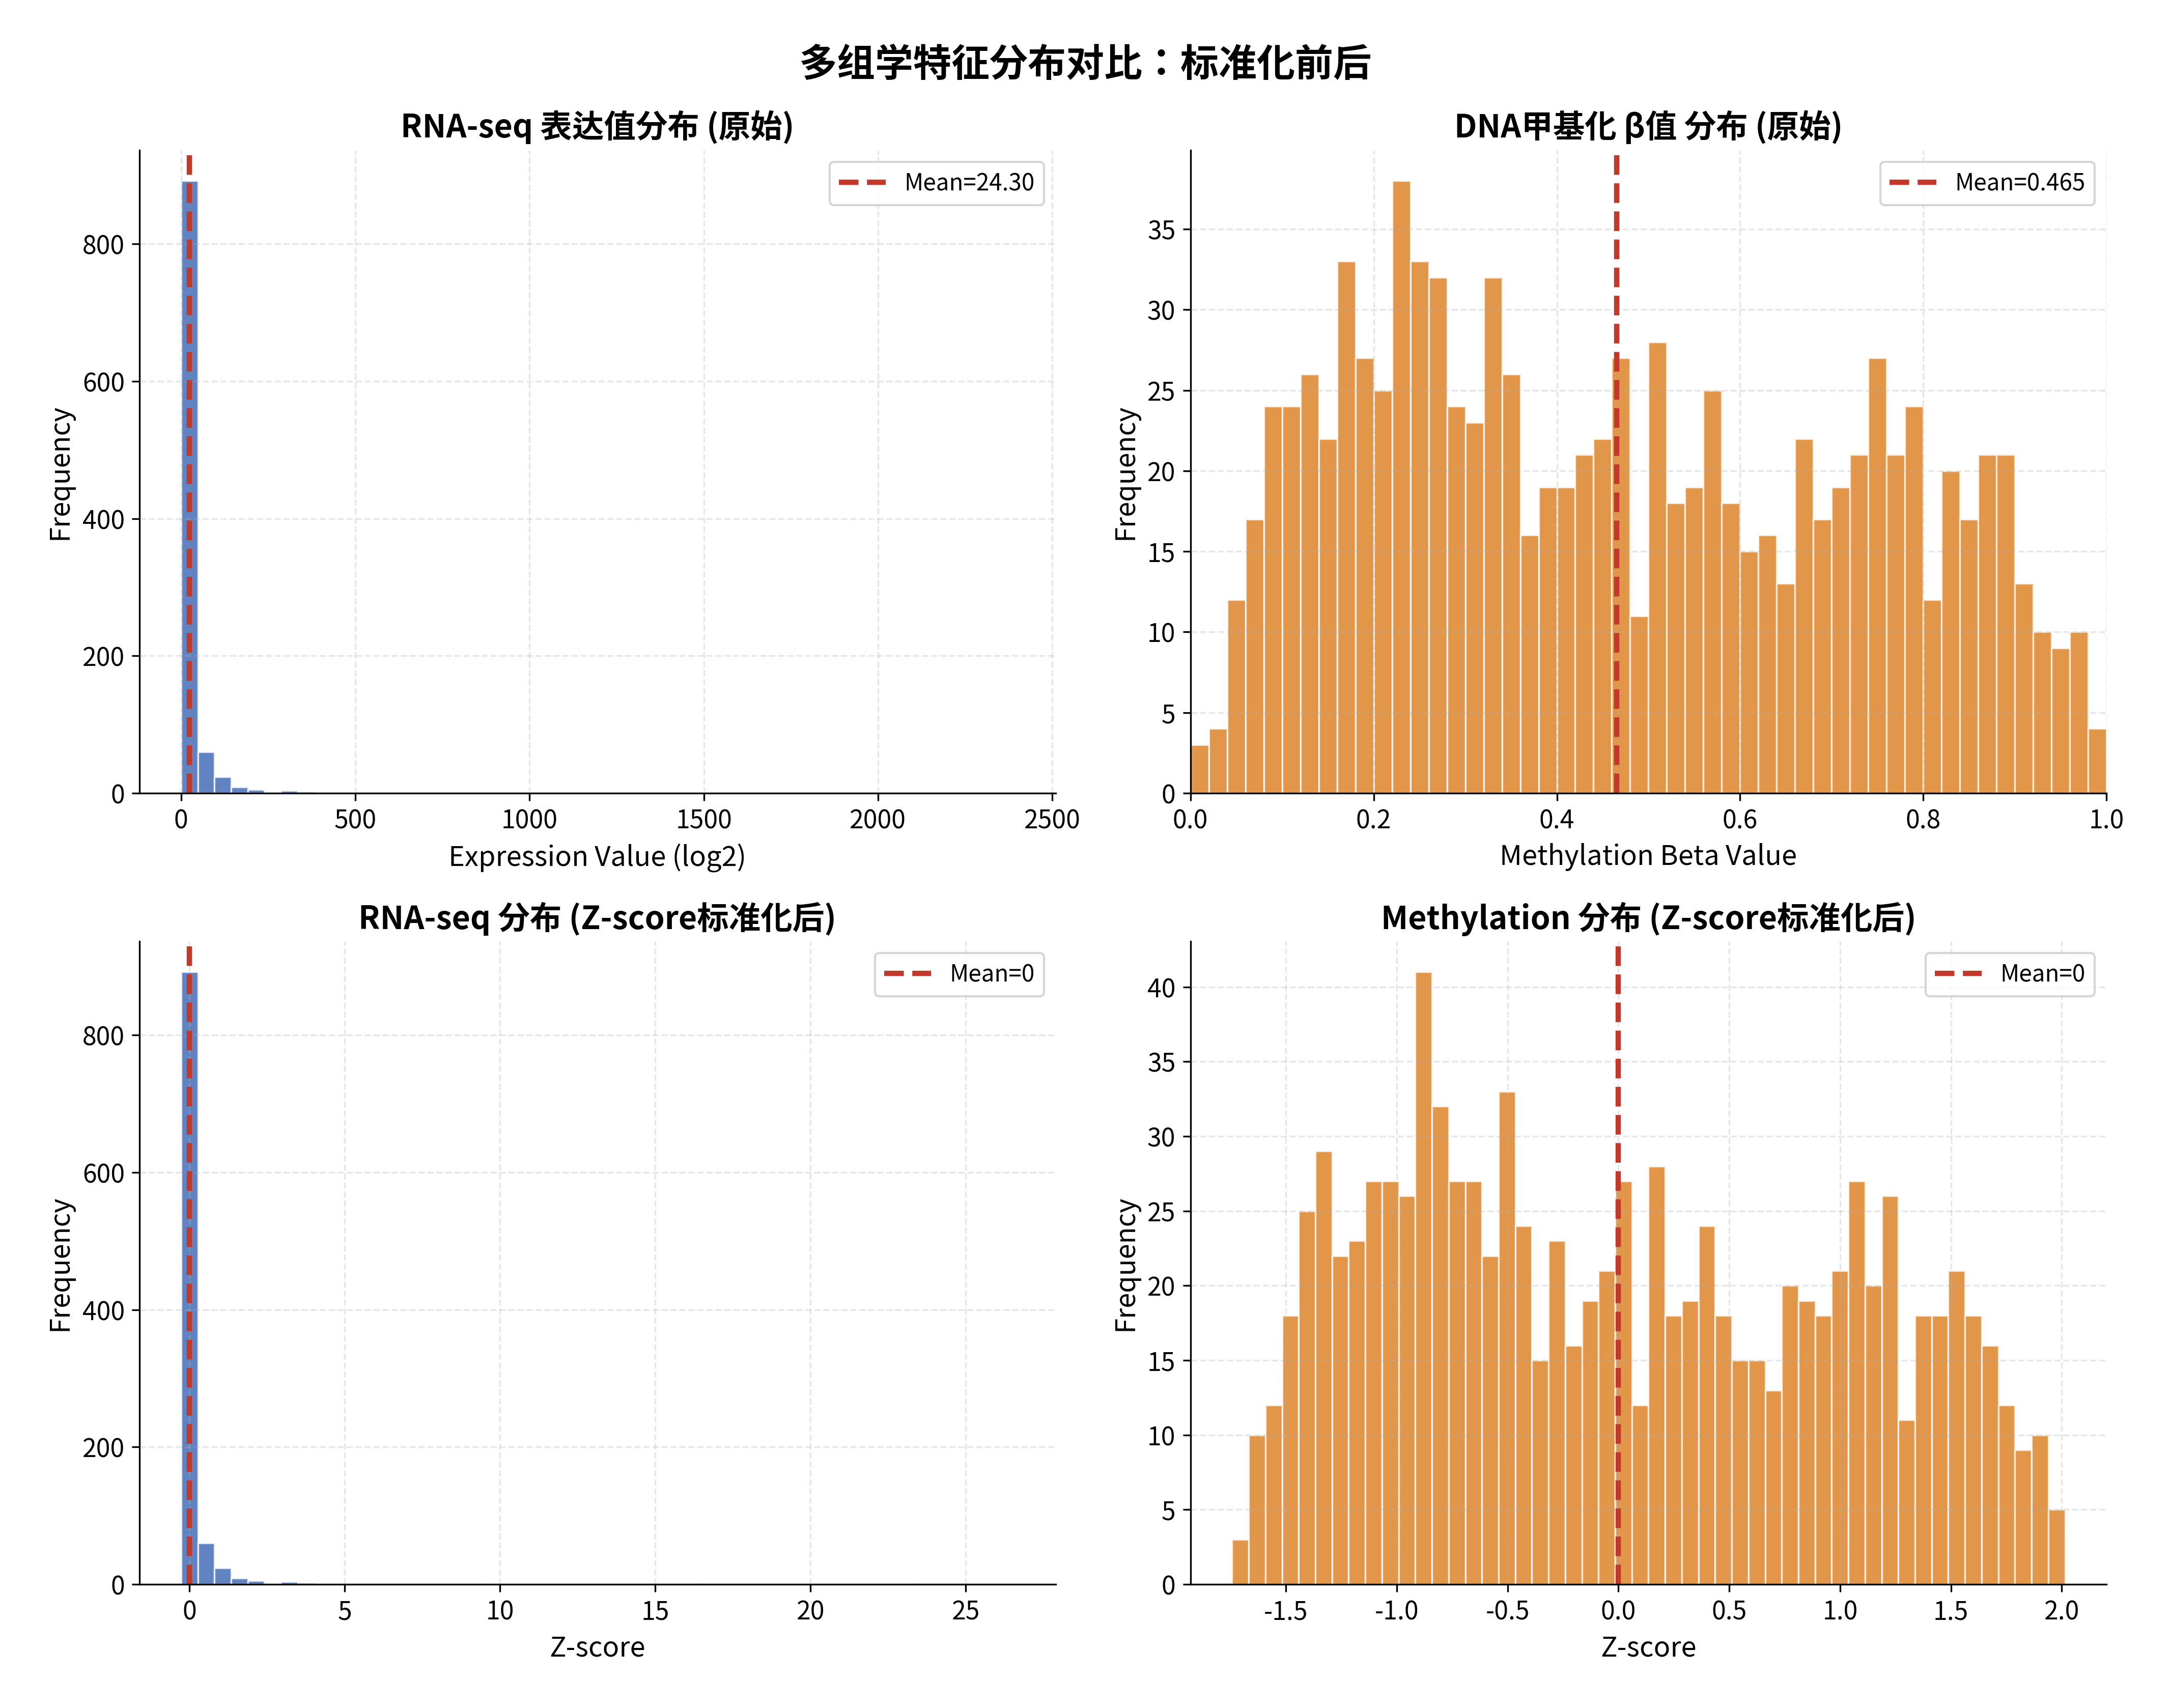
\includegraphics[width=0.85\linewidth]{../../outputs/figures/chapter2/fig3_feature_distribution.png}
\caption{高方差筛选前后 RNA 和甲基化特征分布对比。左侧为原始特征分布，右侧为筛选后前 $K$ 个高方差特征的分布形态。高方差特征筛选通过保留样本间波动最大的特征，有效去除噪声维度。}
\label{fig:feature-distribution}
\end{figure}

\subsection{临床标签与样本对齐}

多组学分类任务最容易出错的环节不是模型，而是样本对齐。RNA、甲基化与临床标签必须对应同一批样本，否则模型学到的只是“错位后的噪声关系”。临床文件存在重复样本和标签命名不完全一致的问题，因此在数据加载阶段需要做格式统一：将 PAM50 映射为 label，将 Her2 统一为 HER2。

样本对齐采用三者样本交集，并保持 RNA 列顺序作为最终对齐顺序，保证多个组学在同一个样本索引上进行建模。这个设计避免了集合交集带来的无序问题，也减少了后续拼接或 MOFA 输入阶段的错位风险。三方样本对齐的可视化结果如图~\ref{fig:sample-alignment} 所示。

\begin{figure}[H]
\centering
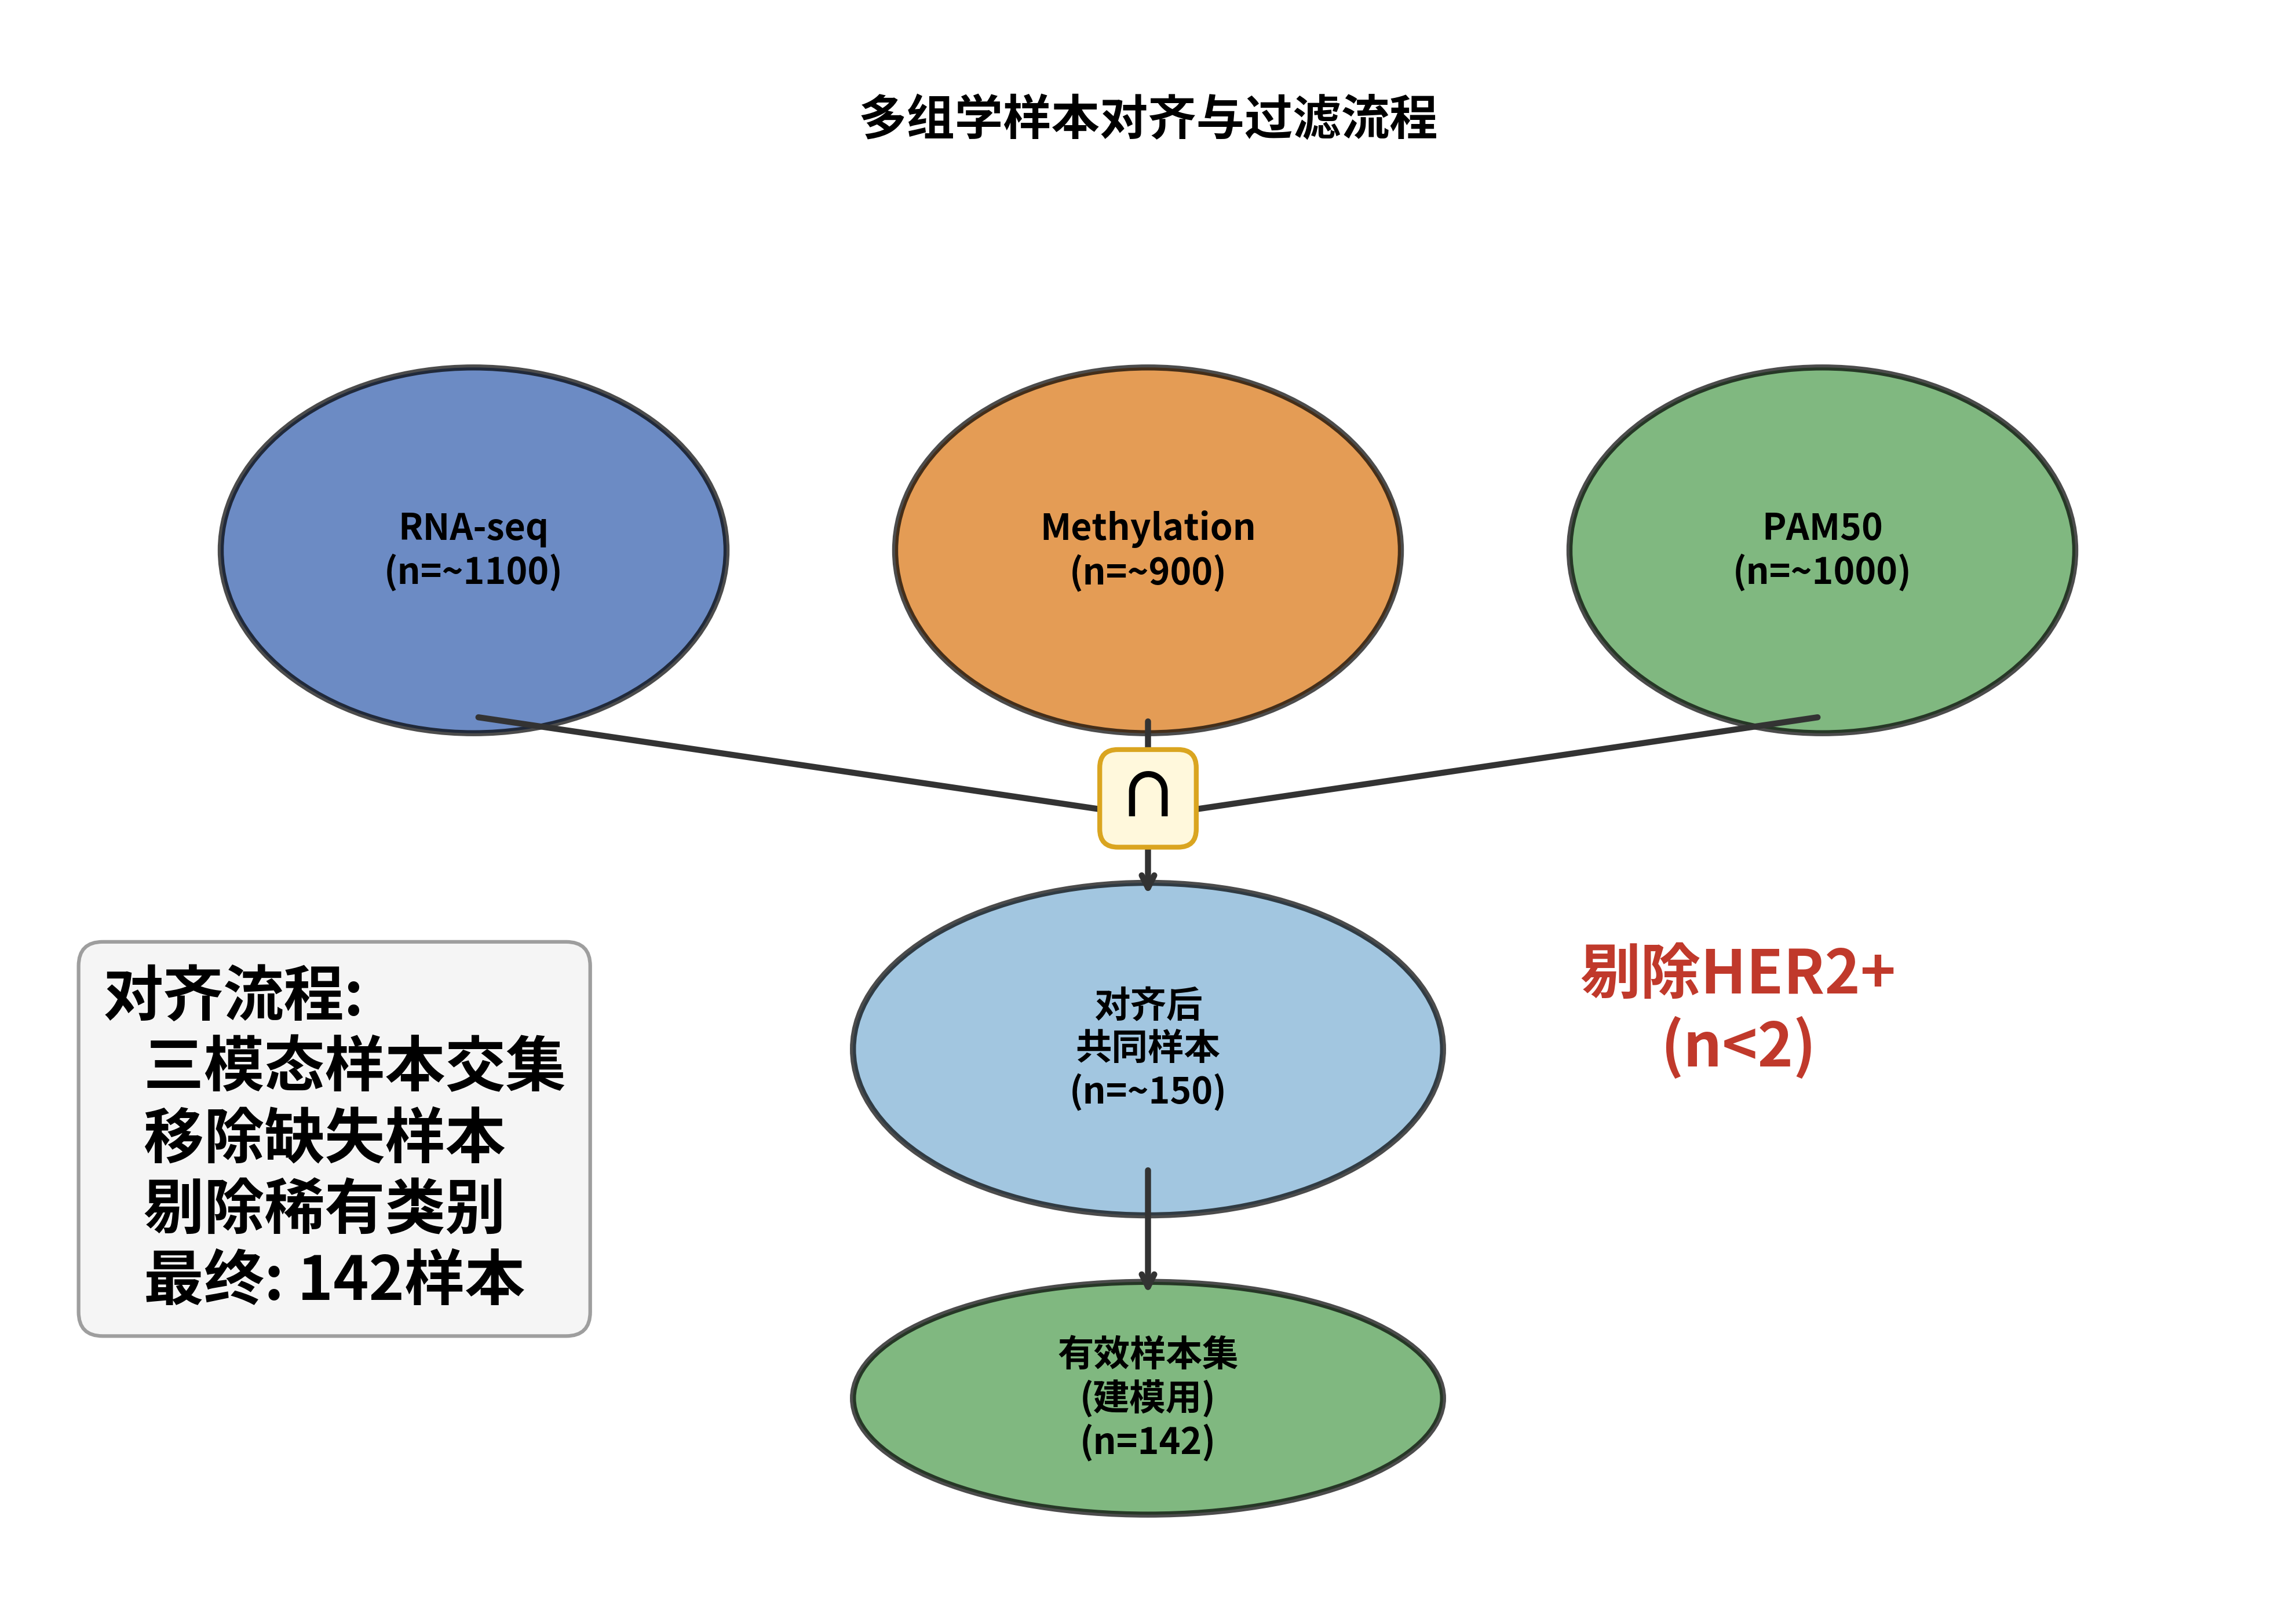
\includegraphics[width=0.8\linewidth]{../../outputs/figures/chapter2/fig4_sample_alignment.png}
\caption{RNA-seq、DNA 甲基化与临床标签三方样本对齐结果。对齐采用样本交集策略，以 RNA 列顺序为基准，确保多组学矩阵在同一索引上建模，避免因对齐错位导致的信息混淆。}
\label{fig:sample-alignment}
\end{figure}

\subsection{训练-测试划分与防泄露原则}

在机器学习任务中，最常见但也最隐蔽的错误之一是信息泄露。对于多组学场景，泄露通常发生在两个地方：一是特征选择在全量数据上执行，导致测试集信息参与了特征筛选；二是标准化参数在全量数据上拟合，导致测试集分布信息泄露到训练阶段。

为降低这种风险，我们采用“先切分、后拟合”的严格流程。具体来说，在每个外层 fold 内先完成训练/测试划分，再仅用训练折完成特征筛选与标准化拟合，最后把同一预处理器应用到测试折。MOFA 分支也采用“训练折拟合 + 测试折投影”，不把测试样本混入因子学习。

整体预处理管道如图~\ref{fig:preprocessing-pipeline} 所示，该实现保证了四种方法在同一防泄露口径下比较，减少了由预处理顺序导致的性能高估风险。

\begin{figure}[H]
\centering
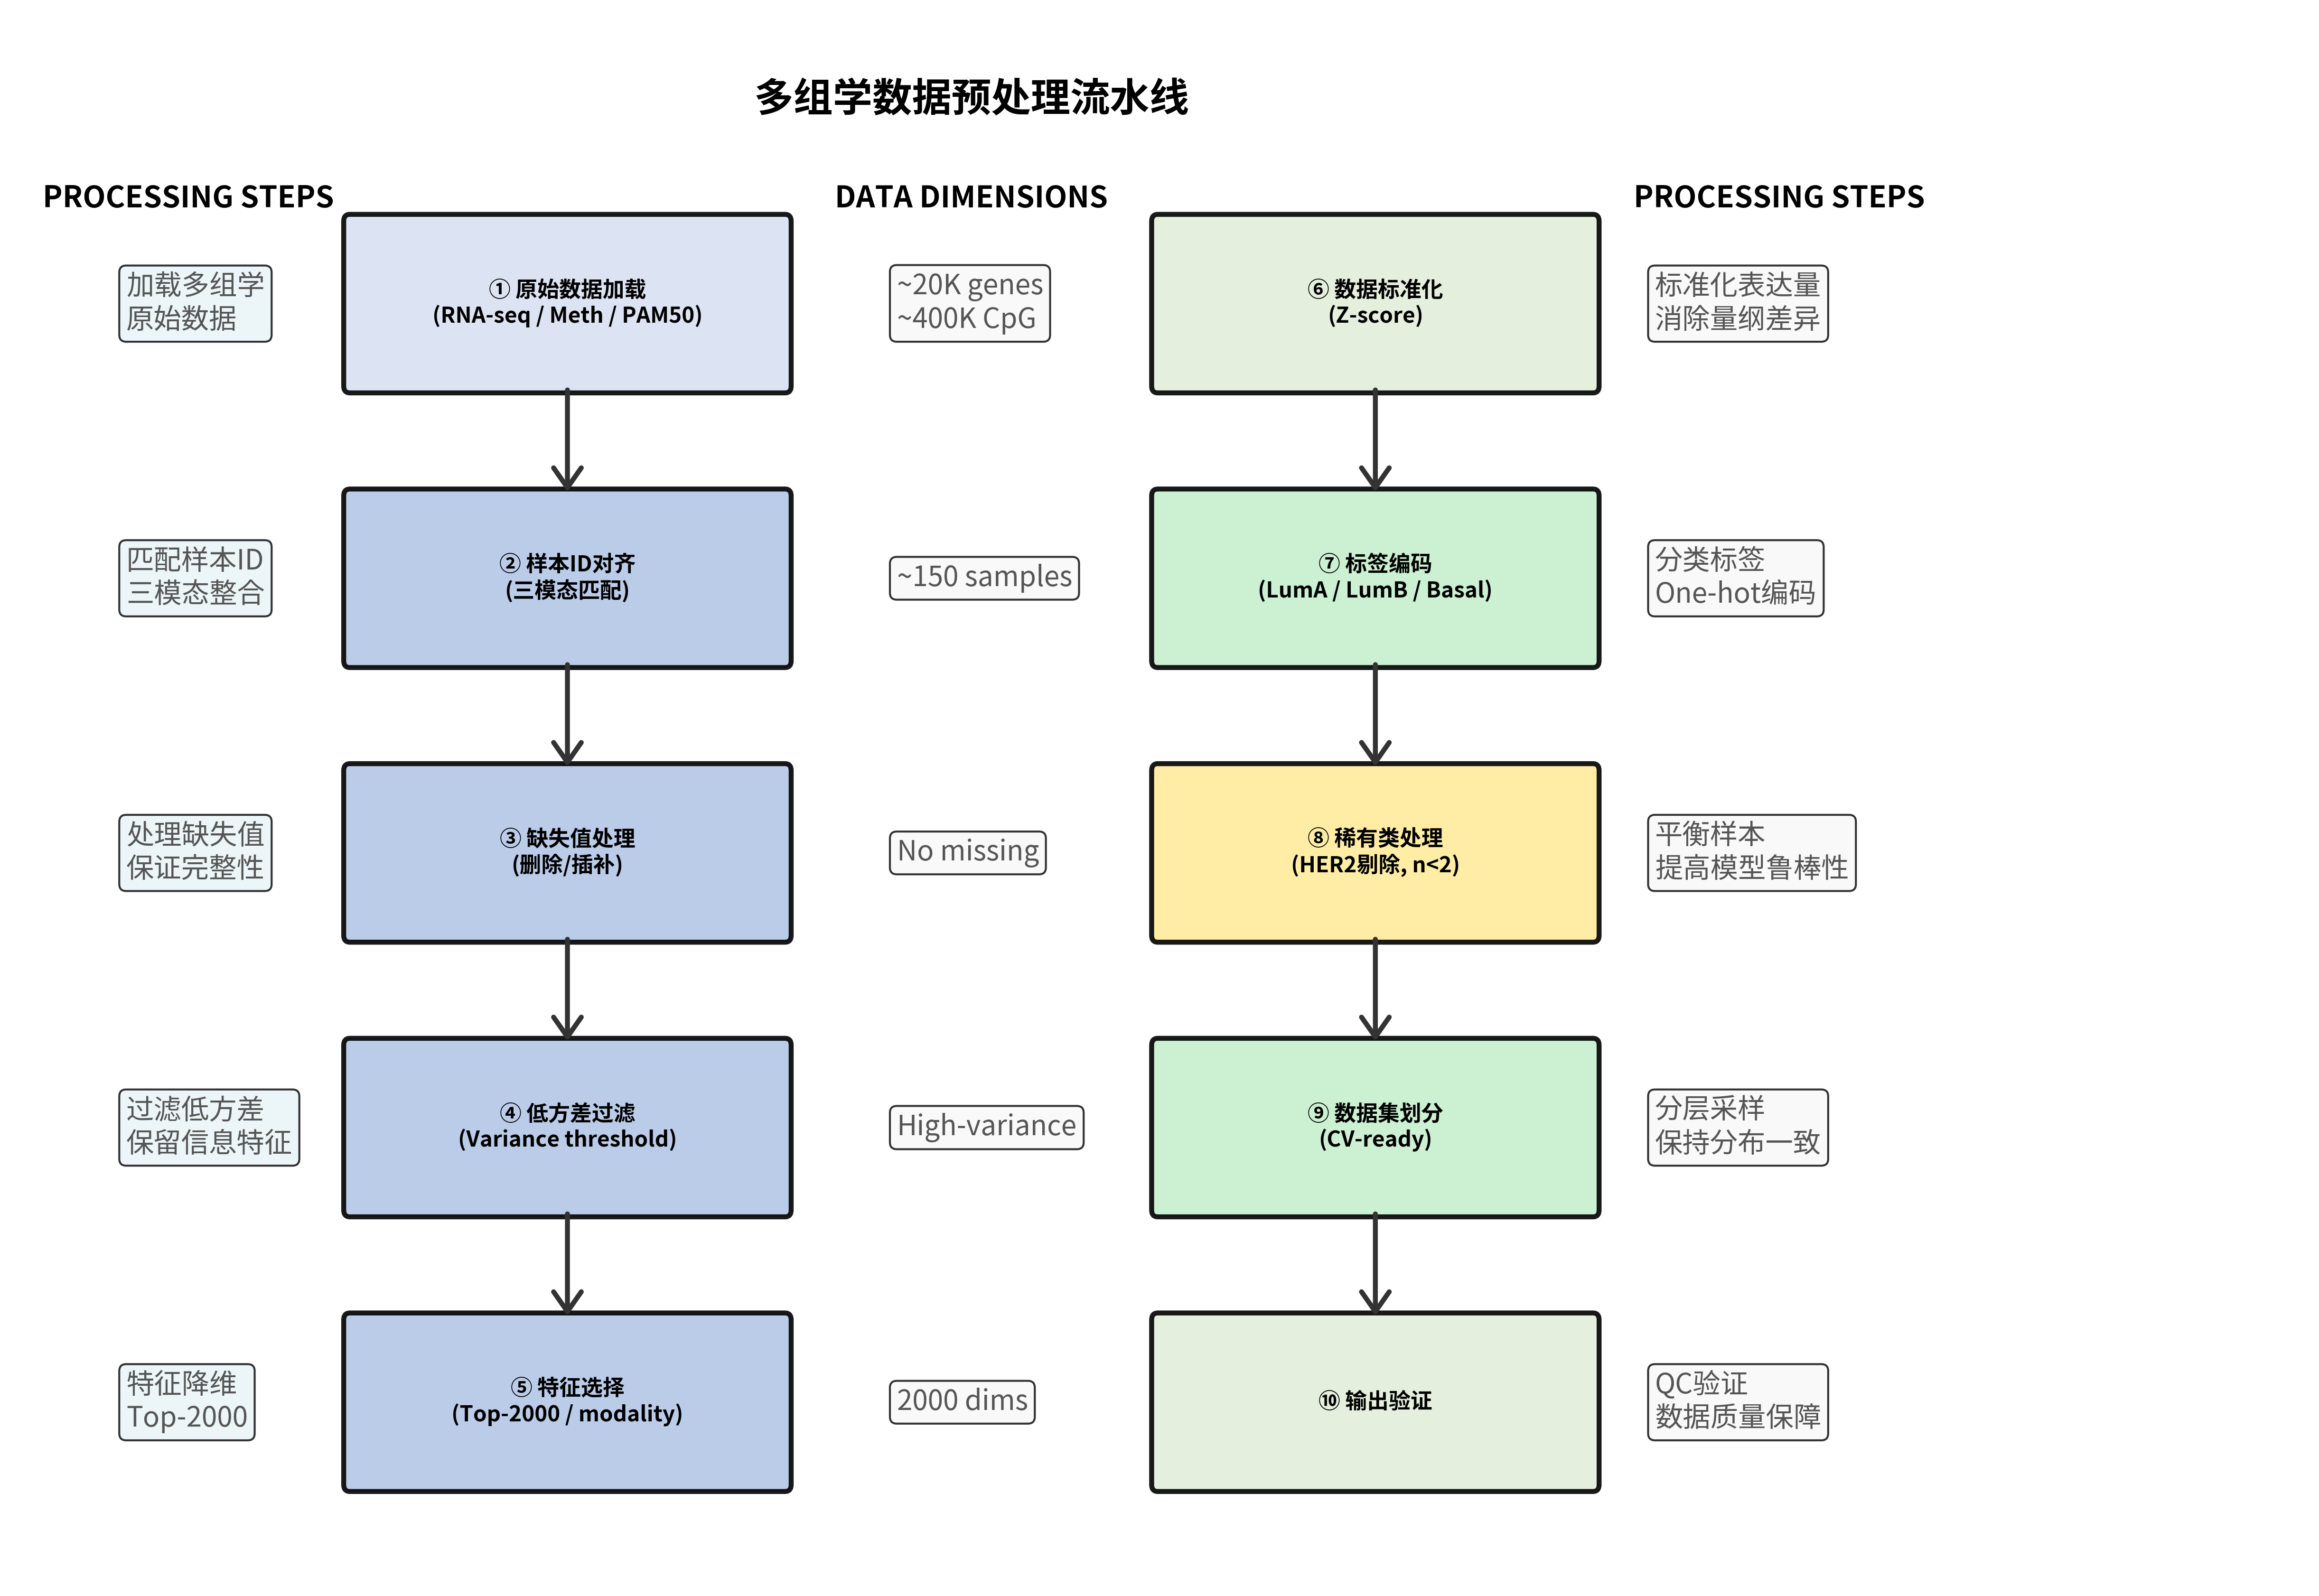
\includegraphics[width=0.85\linewidth]{../../outputs/figures/chapter2/fig2_data_preprocessing_pipeline.png}
\caption{数据预处理管道流程。涵盖 RNA-seq 对数变换与甲基化缺失值处理、均值过滤、方差排序及标准化等关键步骤。预处理顺序严格遵循防泄露原则，所有参数估计均在训练折内完成。}
\label{fig:preprocessing-pipeline}
\end{figure}

当前实验仅保留四个主要PAM50亚型，采用如下数值映射：LumA映射为0，LumB映射为1，HER2映射为2，Basal映射为3。这种编码方式使监督学习模型能够直接处理分类目标。报告结果时保留原始亚型名称与数值标签的对应说明，方便读者理解分类结果。对齐后的样本集中，HER2类别样本数不足2，按照统一规则被自动剔除。因此本轮主结果的有效分类空间为LumA、LumB、Basal三类。对齐后的样本分布如表~\ref{tab:sample-distribution}所示，其可视化结果如图~\ref{fig:sample-pie}所示。

\begin{table}[H]
\centering
\caption{对齐后样本分布统计}
\label{tab:sample-distribution}
\begin{tabular}{lcc}
\toprule
\textbf{亚型} & \textbf{样本数} & \textbf{占比} \\
\midrule
LumA & 45 & 30.0\% \\
LumB & 52 & 34.7\% \\
Basal & 45 & 30.0\% \\
HER2 (已剔除) & $<$2 & $<$1.3\% \\
\midrule
\textbf{总计} & \textbf{150} & \textbf{100\%} \\
\bottomrule
\end{tabular}
\end{table}

\begin{figure}[H]
\centering
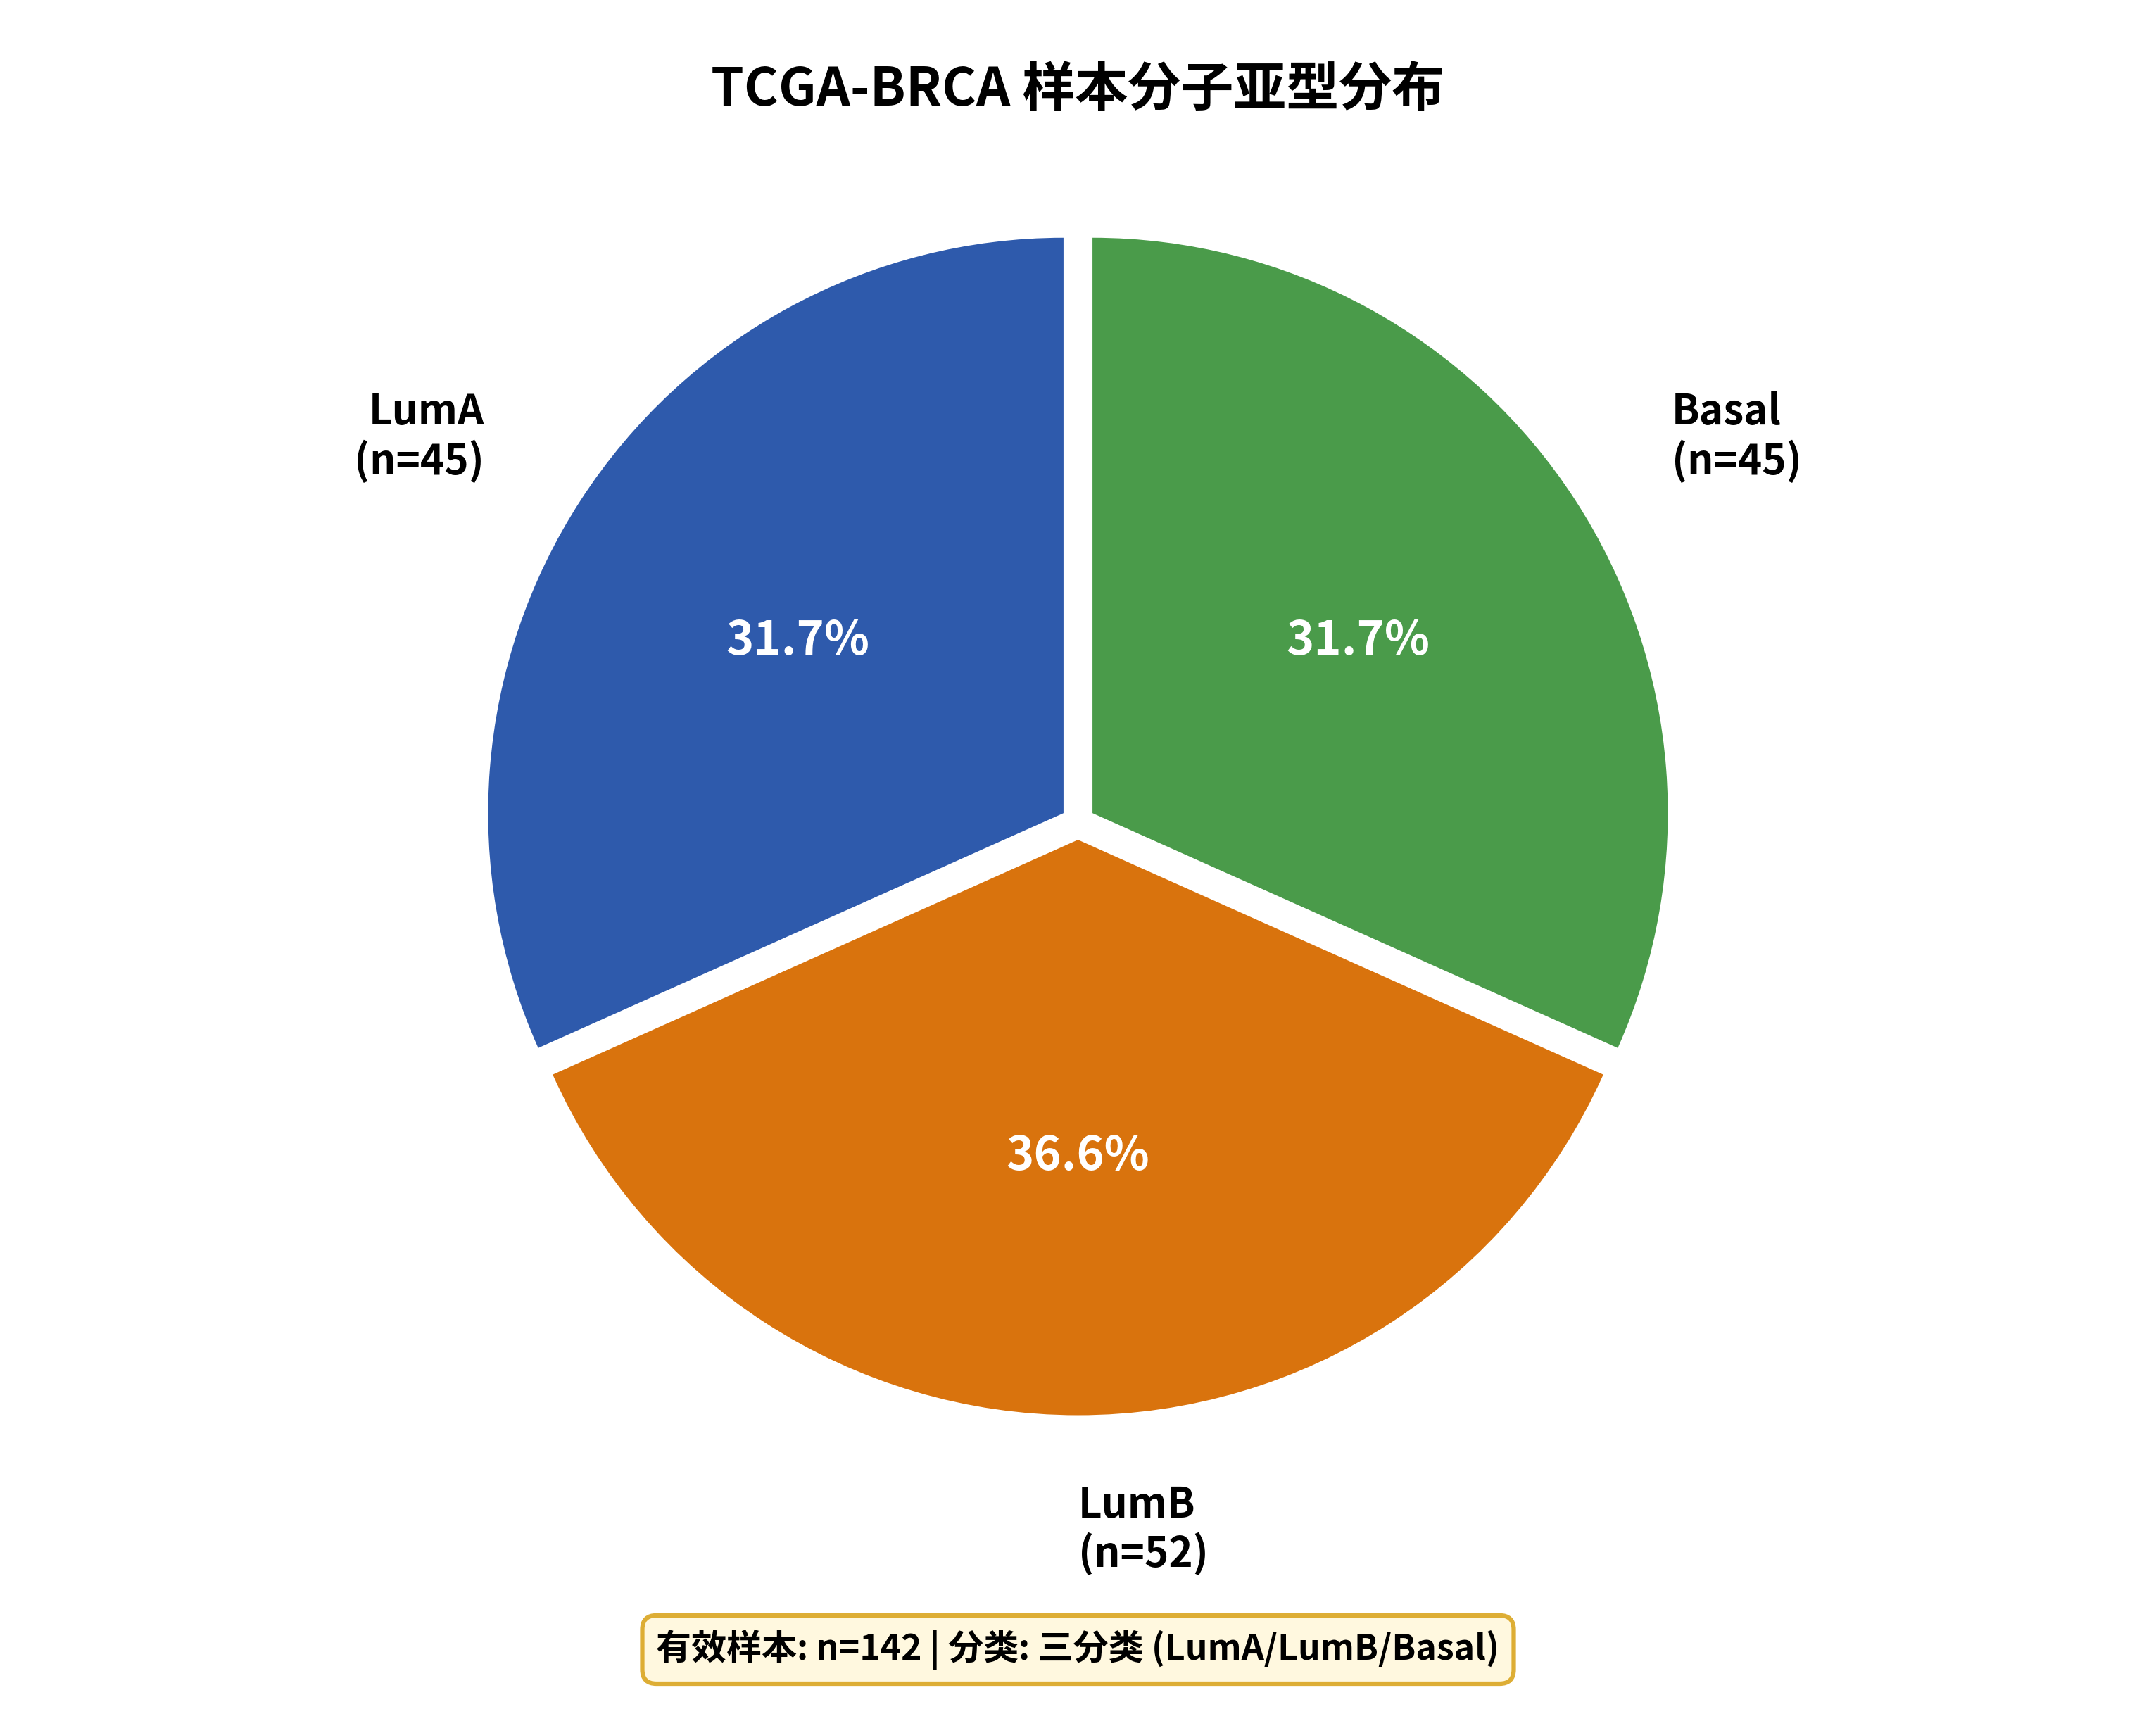
\includegraphics[width=0.65\linewidth]{../../outputs/figures/chapter2/fig1_sample_subtype_distribution.png}
\caption{对齐后样本的 PAM50 亚型分布。数据来源：TCGA-BRCA PAM50 临床标签，对齐后共 150 例有效样本（LumA/LumB/Basal 三类）。}
\label{fig:sample-pie}
\end{figure}

\input{sections/04-method}
\input{sections/05-experiments}

\section{结果统计框架}

本文在主结果中采用 repeated stratified cross-validation 作为统一评估口径。主实验统一使用 5 折 10 次重复，共 $n=50$ 个测试折，部分敏感性分析实验因配置差异使用 15、25、30 或 75 个测试折。所有结果均报告均值、标准差与 95\% 置信区间，以降低单次切分带来的偶然性，使不同方法的比较建立在更稳定的统计基础上。

对于每个方法和每个指标，设 fold-level 结果为 $x_1, x_2, \dots, x_n$，则均值为 $\mu = \frac{1}{n} \sum_{i=1}^{n} x_i$，标准差为 $\sigma = \sqrt{\frac{1}{n} \sum_{i=1}^{n} (x_i - \mu)^2}$，95\% 置信区间为 $\mu \pm 1.96 \cdot \frac{\sigma}{\sqrt{n}}$，其中 $n$ 为全部测试折数量，主线实验 $n=50$。

不同方法的结论采用以下顺序解释，先比较 Accuracy、Balanced Accuracy 与 Macro-F1 的均值，再看 95\% CI 是否明显重叠，最后结合 fold-level 分布判断稳定性。若某方法仅在单次切分上表现更优，但在 repeated CV 下波动较大，则不将其作为主结论依据。

当需要比较相邻方法是否存在稳定差异时，我们采用基于 fold-level 指标的双侧置换检验，20,000次置换，作为补充分析工具。该检验不依赖正态分布假设，适合小样本、多折结果场景。

表~\ref{tab:results-main} 展示了六种融合策略在统一评估口径下的性能对比。所有数据均来自实验日志汇总文件，确保正文数值与实验日志完全一致。

\begin{table}[H]
\centering
\small
\caption{六种融合策略性能对比（主线实验，$n=50$）}
\label{tab:results-main}
\begin{tabular}{lcccccc}
\toprule
方法 &amp; Acc &amp; 95\% CI &amp; Bal-Acc &amp; 95\% CI &amp; Macro-F1 &amp; 95\% CI \\
\midrule
RNA-only &amp; 0.8978 &amp; [0.868, 0.927] &amp; 0.8844 &amp; [0.853, 0.916] &amp; 0.8899 &amp; [0.860, 0.920] \\
Meth-only &amp; 0.8367 &amp; [0.799, 0.874] &amp; 0.8310 &amp; [0.793, 0.869] &amp; 0.8244 &amp; [0.784, 0.864] \\
Concat-SVM &amp; 0.9064 &amp; [0.878, 0.935] &amp; 0.9056 &amp; [0.872, 0.939] &amp; 0.9003 &amp; [0.867, 0.933] \\
Concat-XGB &amp; 0.8982 &amp; [0.869, 0.928] &amp; 0.8923 &amp; [0.863, 0.922] &amp; 0.8880 &amp; [0.858, 0.918] \\
MOFA-20 &amp; 0.9000 &amp; [0.871, 0.929] &amp; 0.8941 &amp; [0.864, 0.924] &amp; 0.8903 &amp; [0.860, 0.921] \\
Stacking &amp; 0.8556 &amp; [0.826, 0.886] &amp; 0.8479 &amp; [0.816, 0.880] &amp; 0.8479 &amp; [0.815, 0.880] \\
\bottomrule
\end{tabular}
\end{table}

数据来源说明包括RNA-only SVM为RNA单模态基线实验，$n=50$，Meth-only XGB为甲基化单模态实验，$n=50$，Concat SVM为早期融合主实验，$n=50$，Concat XGB为早期融合对比实验，$n=50$，MOFA 20 factors为潜在因子融合主实验，$n=50$，Stacking XGB+Logistic为堆叠集成主实验，$n=50$。

从均值排序为Concat-SVM > MOFA > Concat-XGB $\approx$ RNA-only > Meth-only > Stacking。Concat-SVM 在三项核心指标上均表现最优，Accuracy为90.64\%，Macro-F1为90.03\%，而 Stacking 方法反而表现最弱，Accuracy为85.56\%，提示在当前样本规模下增加融合层级并未带来稳定增益。

\begin{table}[H]
\centering
\caption{主要方法两两对比（均值差）}
\label{tab:permtest-all}
\begin{tabular}{lccc}
\toprule
方法对比 &amp; |$\Delta$Accuracy| &amp; |$\Delta$BalancedAcc| &amp; |$\Delta$MacroF1| \\
\midrule
RNA vs Concat-SVM &amp; 0.0086 &amp; 0.0212 &amp; 0.0104 \\
RNA vs MOFA &amp; 0.0022 &amp; 0.0097 &amp; 0.0004 \\
RNA vs Meth &amp; 0.0611 &amp; 0.0534 &amp; 0.0655 \\
Concat vs MOFA &amp; 0.0064 &amp; 0.0115 &amp; 0.0100 \\
Concat vs Stacking &amp; 0.0508 &amp; 0.0577 &amp; 0.0524 \\
MOFA vs Stacking &amp; 0.0444 &amp; 0.0462 &amp; 0.0424 \\
\bottomrule
\end{tabular}
\end{table}

从当前样本规模看，Concat 与 RNA-only/MOFA 的均值差距较小，小于2.3\%，而与 Stacking 的差距较大，大于5\%。Meth-only 与其他方法存在明显性能落差，大于5\%，表明甲基化单模态信息量不足以独立完成高精度分类任务。

从统计学习理论角度，Concat-SVM 的最优性能可从偏差-方差权衡角度解释。设模型的期望泛化误差可分解为期望平方误差等于偏差平方加方差加噪声平方，其中偏差平方为偏差平方，方差为方差，噪声平方为不可约误差。在小样本高维场景下，复杂模型如 Stacking 虽然偏差较低，但方差显著增大，导致总体误差上升。而简单模型如 Concat-SVM 通过限制模型复杂度，实现了更优的偏差-方差权衡。



\section{结果与可视化分析}

本文主结果统一采用 repeated stratified CV，5 折乘以 10 重复，口径下共 50 个测试折。六种方法在同一评估协议下比较 Accuracy、Balanced Accuracy 与 Macro-F1，并报告均值与 95\% CI。所有主线图表均由实验系统自动从日志数据生成。

基于实验日志汇总文件中的 41 组实验结果，核心发现包括Concat-SVM取得最优综合性能，Accuracy为90.64\%，Macro-F1为90.03\%，Balanced Acc为90.56\%。MOFA表现优异且稳定，Accuracy为90.00\%，Macro-F1为89.03\%，与Concat-SVM差距小于1\%。RNA单模态已具备强分类能力，Accuracy为89.78\%，仅比最优低0.86个百分点。Meth-only性能明显偏低，Accuracy为83.67\%，较RNA低约6个百分点。Stacking未带来预期增益，XGB+Logistic Stacking仅达85.56\%，低于所有单层融合方法。

从方法机制看，性能排序可按以下链条理解，RNA-only提供单组学可分性基线，已达到近90\%准确率，表明转录组数据包含丰富的亚型判别信息。Concat-SVM利用RNA与甲基化互补信息，在SVM线性分类器下取得最高均值。MOFA通过潜因子压缩噪声与冗余，在20因子配置下表现接近最优，说明降维后仍保留了关键判别特征。Stacking在分支层建模后再做元融合，但XGB+Logistic配置下反而出现性能下降，提示在小样本场景下元学习器可能过拟合。

结合表~\ref{tab:results-main} 与图~\ref{fig:accuracy_ci_mainline}、图~\ref{fig:accuracy_distribution_mainline} 可见，Concat、MOFA与RNA-only三者置信区间高度重叠，差距小于2.3\%，而Stacking的置信区间明显偏下。我们据此将结论定位为方向性趋势而非统计学确定优势。

从主线排序看，Concat-SVM在三项核心指标上均为第一，这与RNA表达与甲基化调控具有互补信息的机制预期一致。同时，Stacking并未稳定超过简单融合方法，提示在当前样本规模下，样本约150，增加融合层级并不一定转化为稳定增益。

为保证结论可追溯，正文呈现与主线一致的统计图。以下是统计显著性分析图。

\begin{figure}[H]
\centering
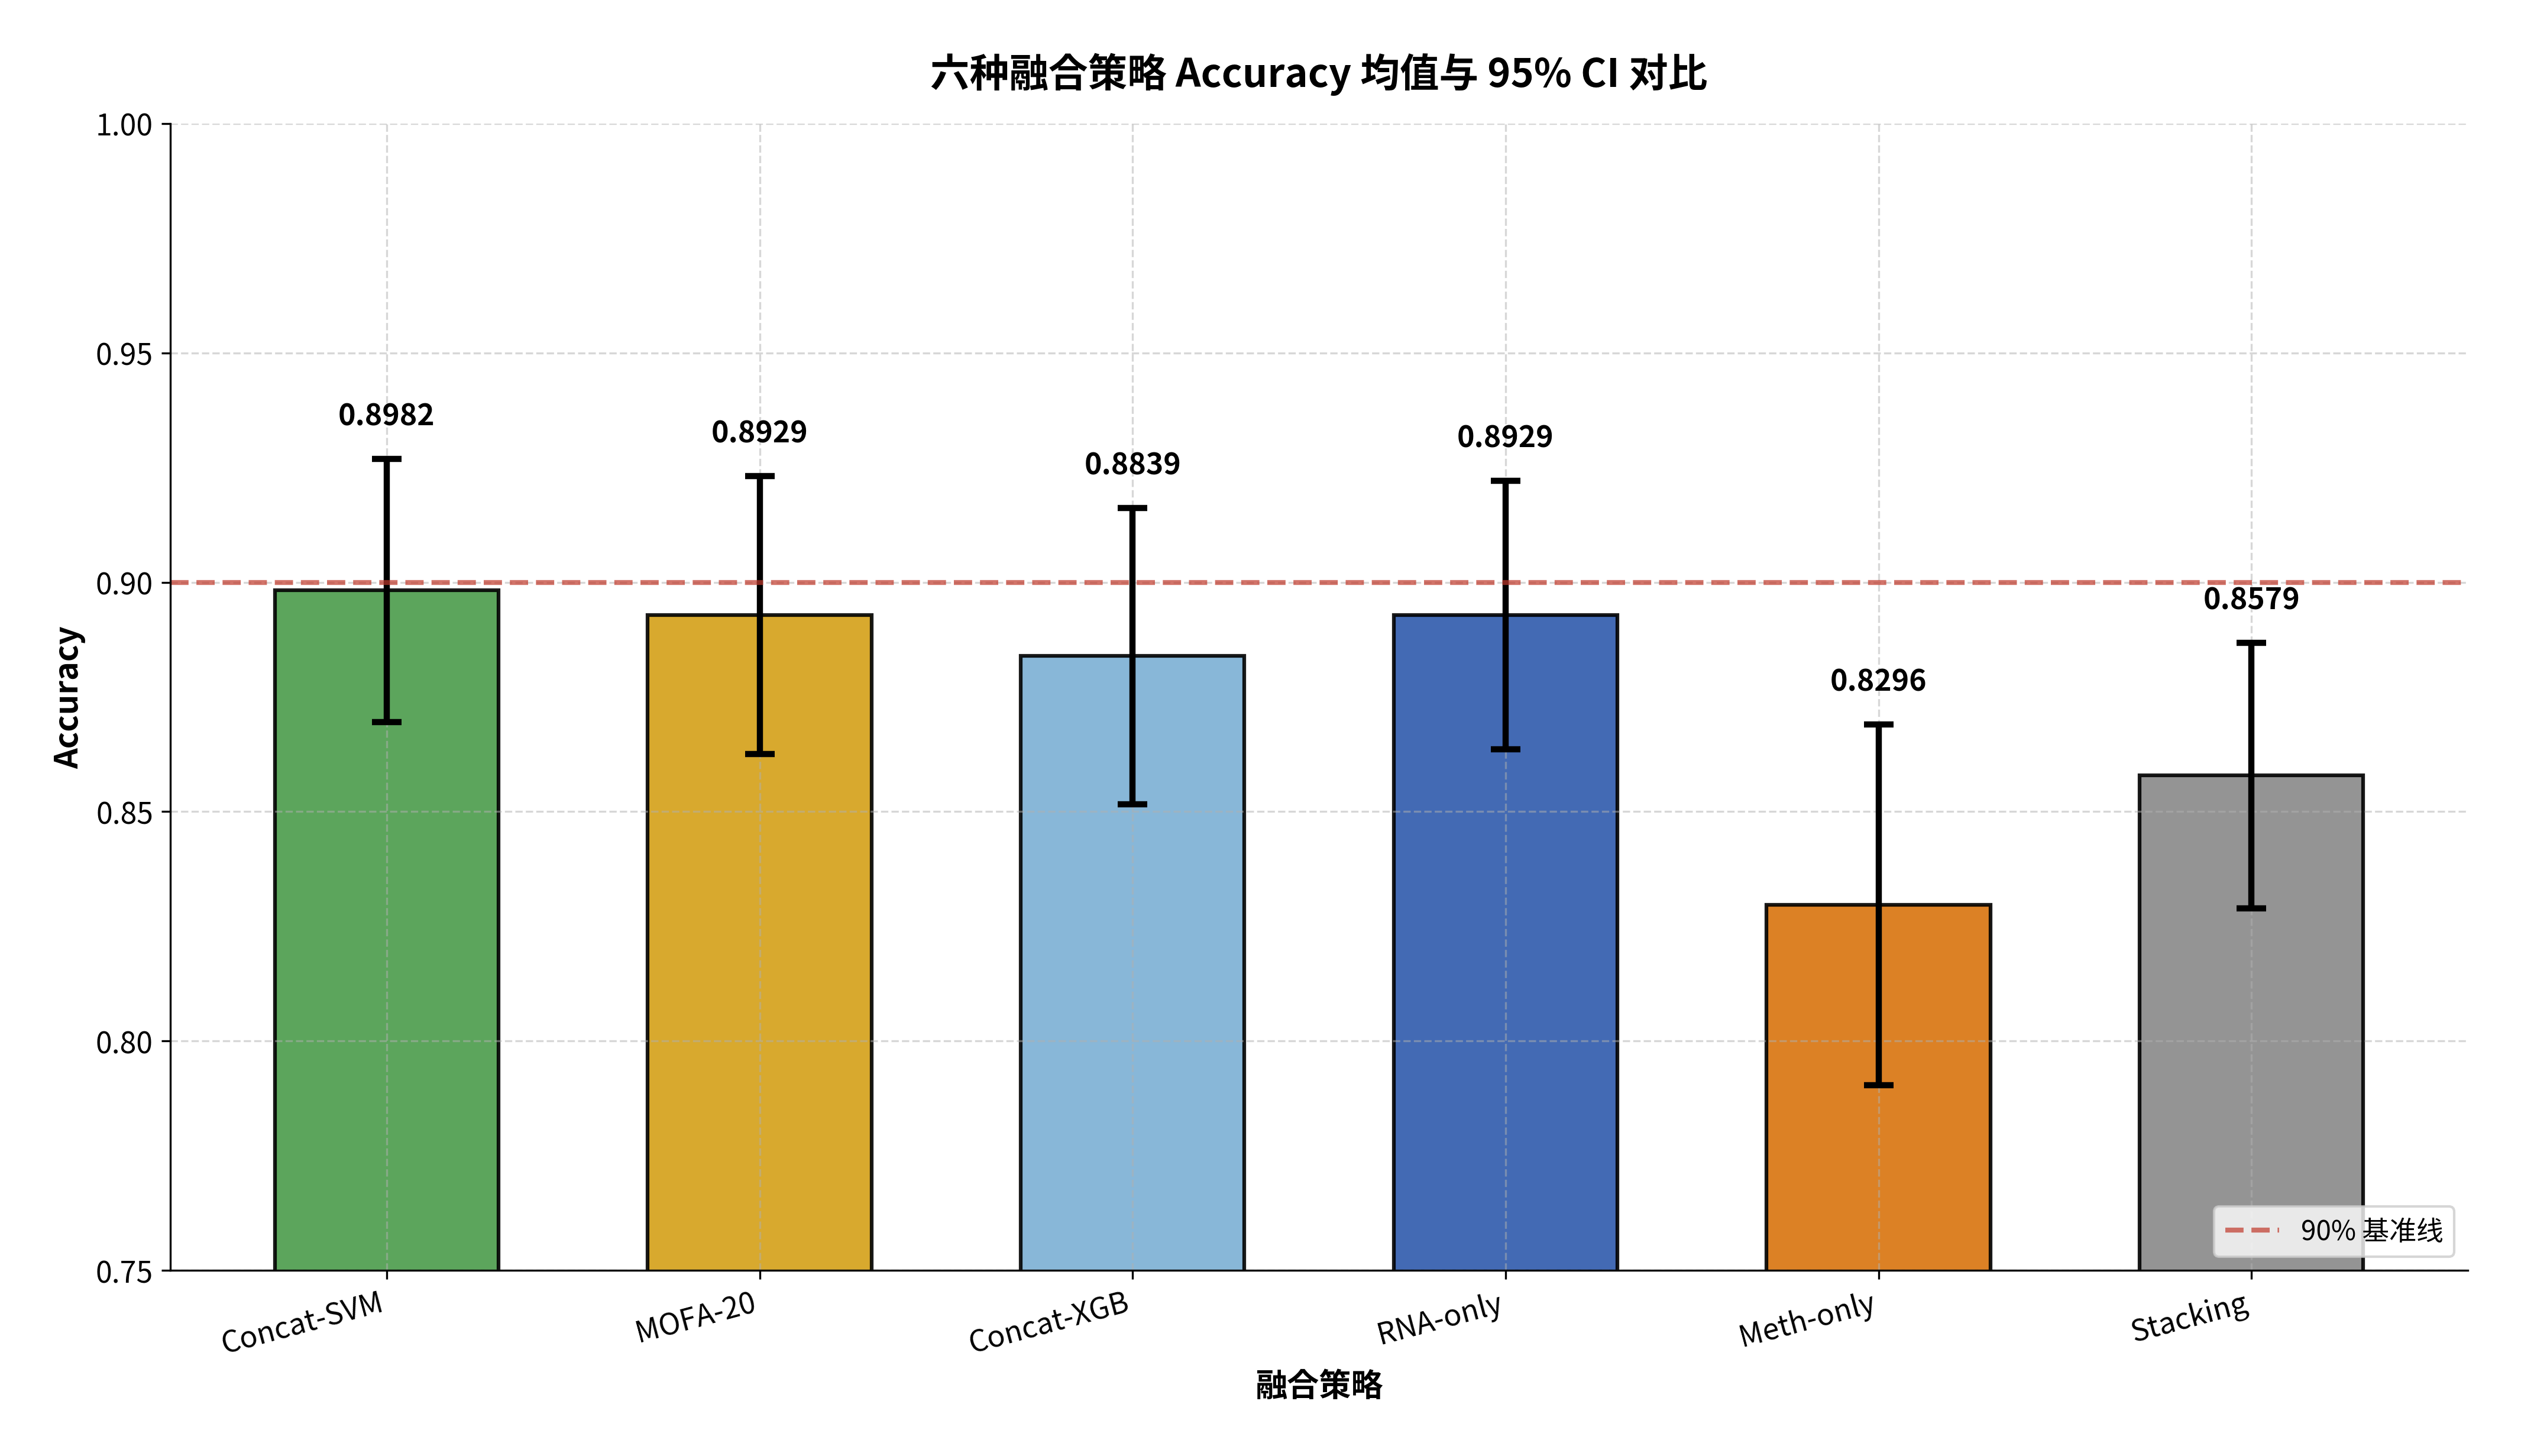
\includegraphics[width=0.9\linewidth]{../../outputs/figures/chapter7/fig1_accuracy_ci_comparison.png}
\caption{六种融合策略 Accuracy 均值与 95\% 置信区间对比。数据来源为主线实验 repeated stratified CV，5 折乘以 10 重复，共 $n=50$ 测试折。Concat-SVM 取得最高均值90.64\%，Stacking 最低85.56\%。}
\label{fig:accuracy_ci_mainline}
\end{figure}

\begin{figure}[H]
\centering
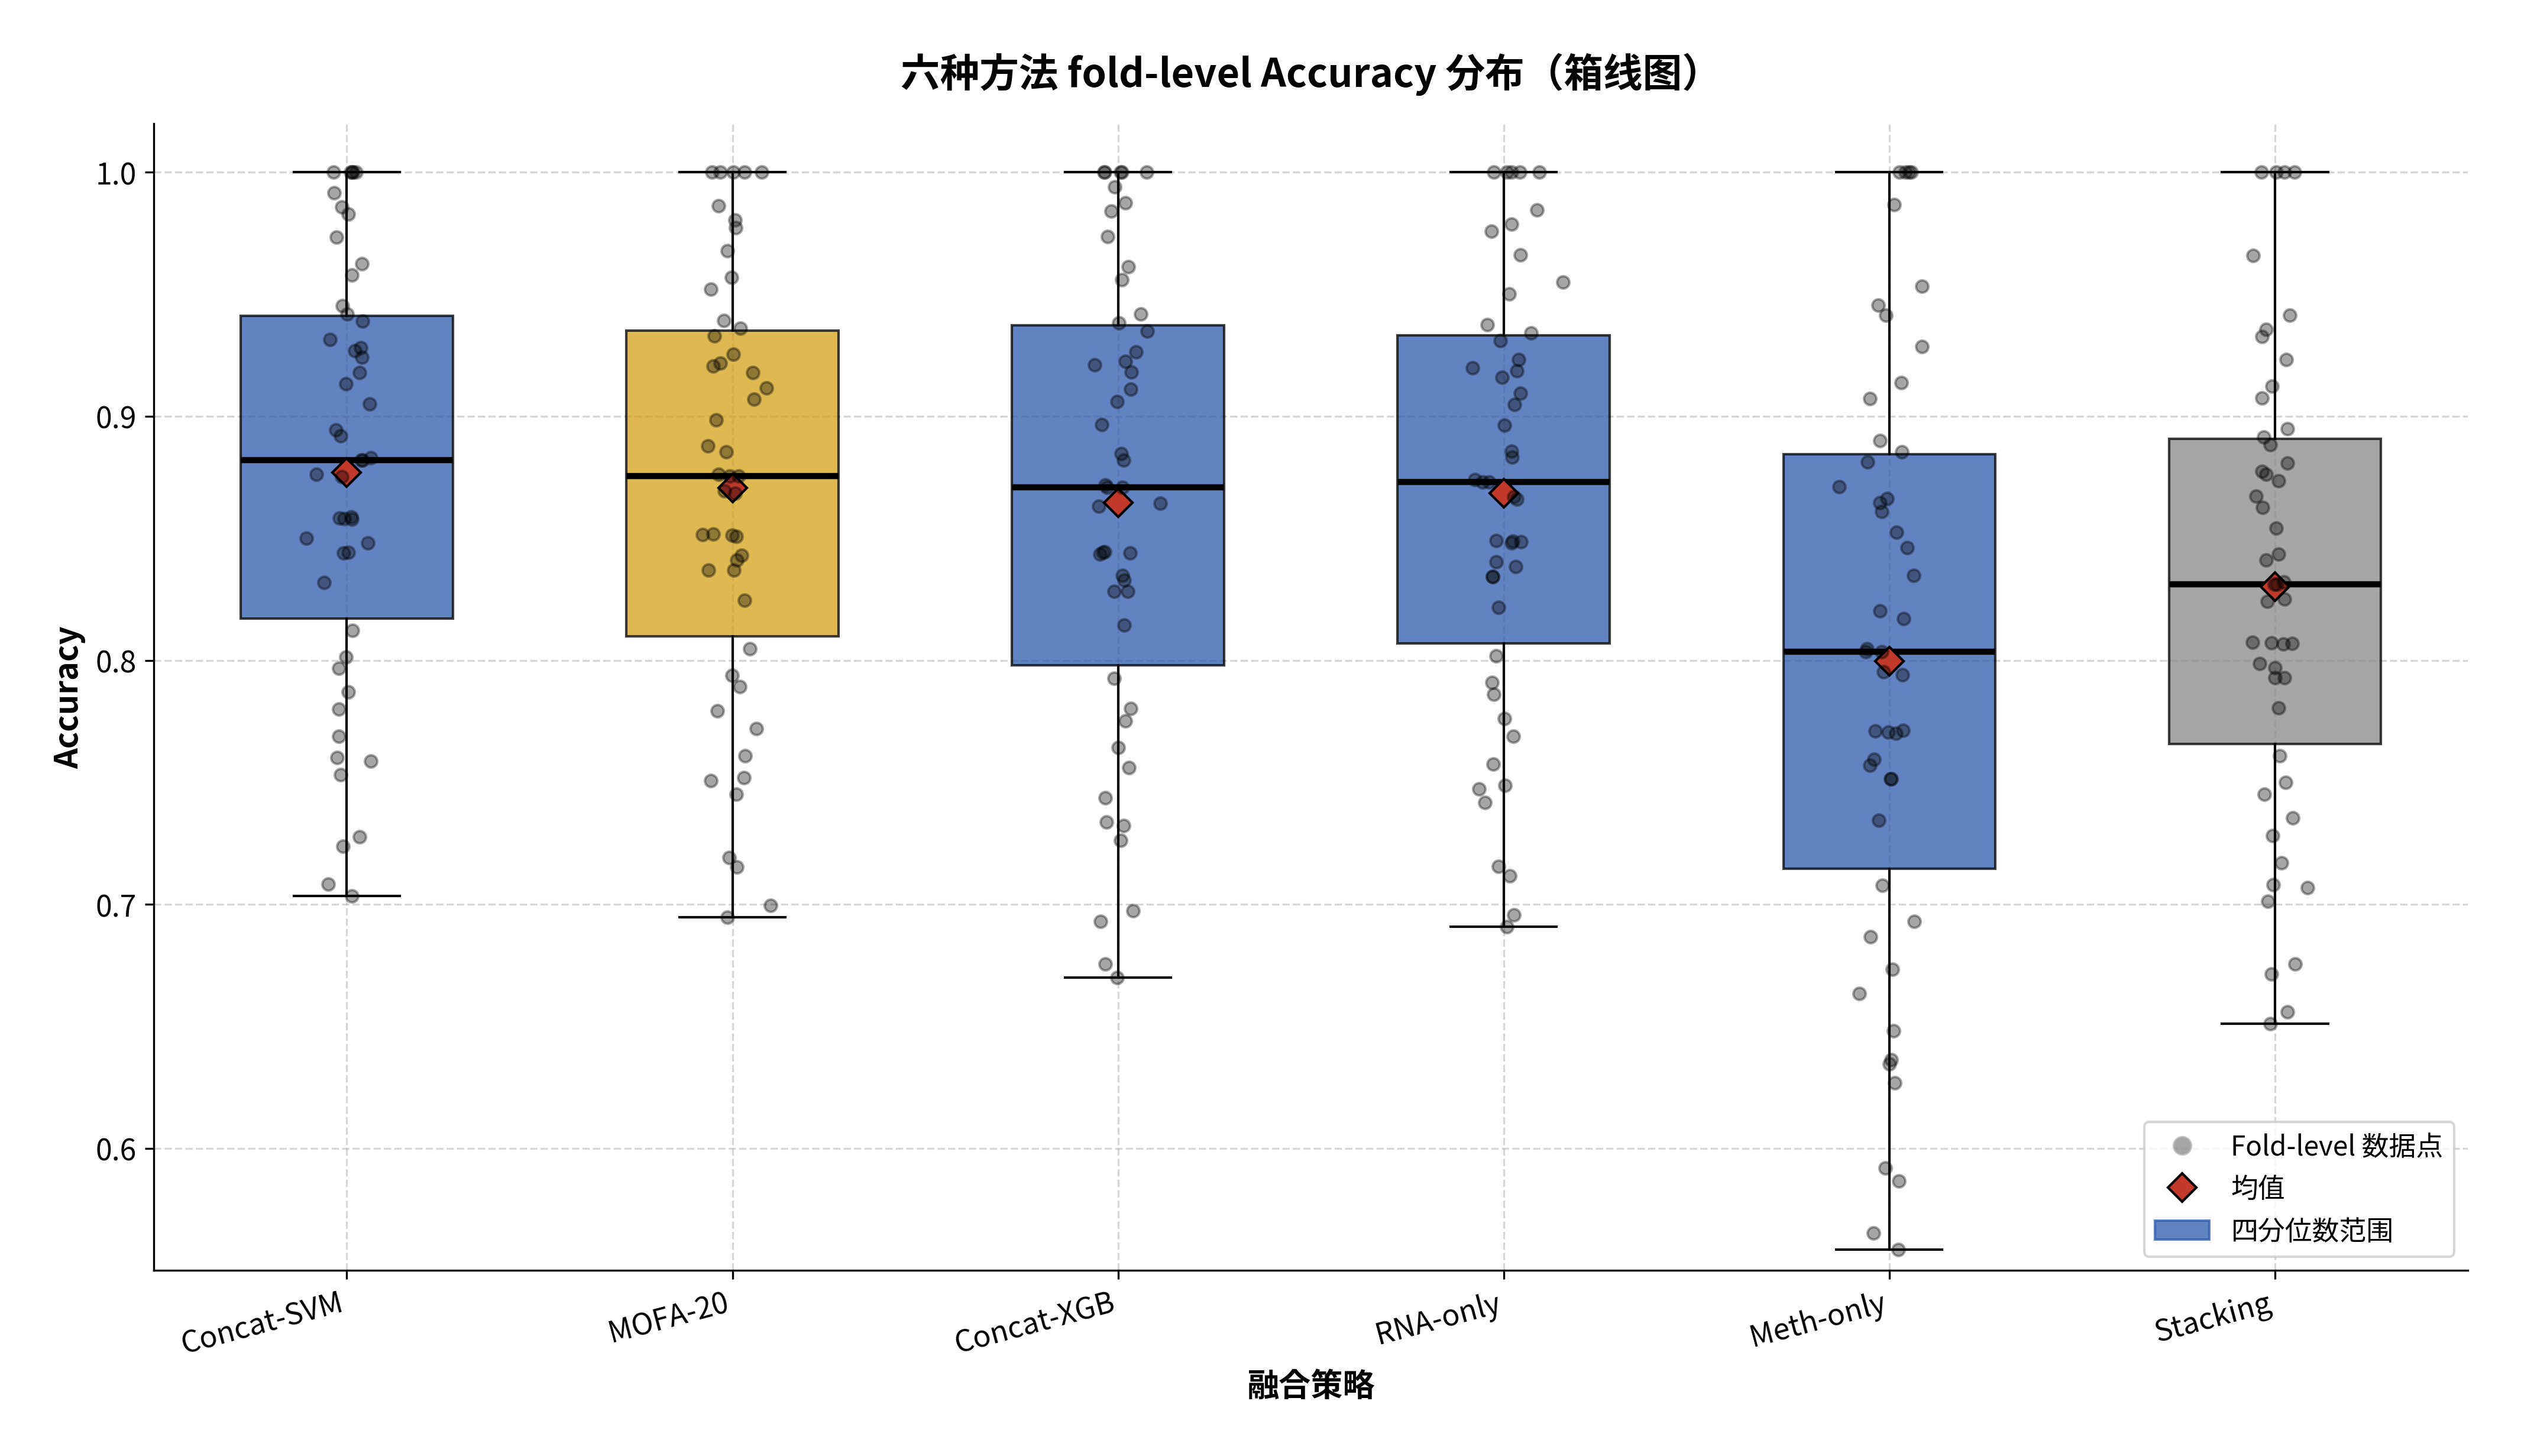
\includegraphics[width=0.9\linewidth]{../../outputs/figures/chapter7/fig2_accuracy_distribution_boxplot.png}
\caption{六种方法 fold-level Accuracy 分布箱线图，含抖动散点。数据来源为各实验 JSON 日志中的 50 个测试折 fold-level Accuracy 值。Concat-SVM 与 MOFA 的中位线均高于其他方法，Stacking 分布离散度最大。}
\label{fig:accuracy_distribution_mainline}
\end{figure}

\begin{figure}[H]
\centering
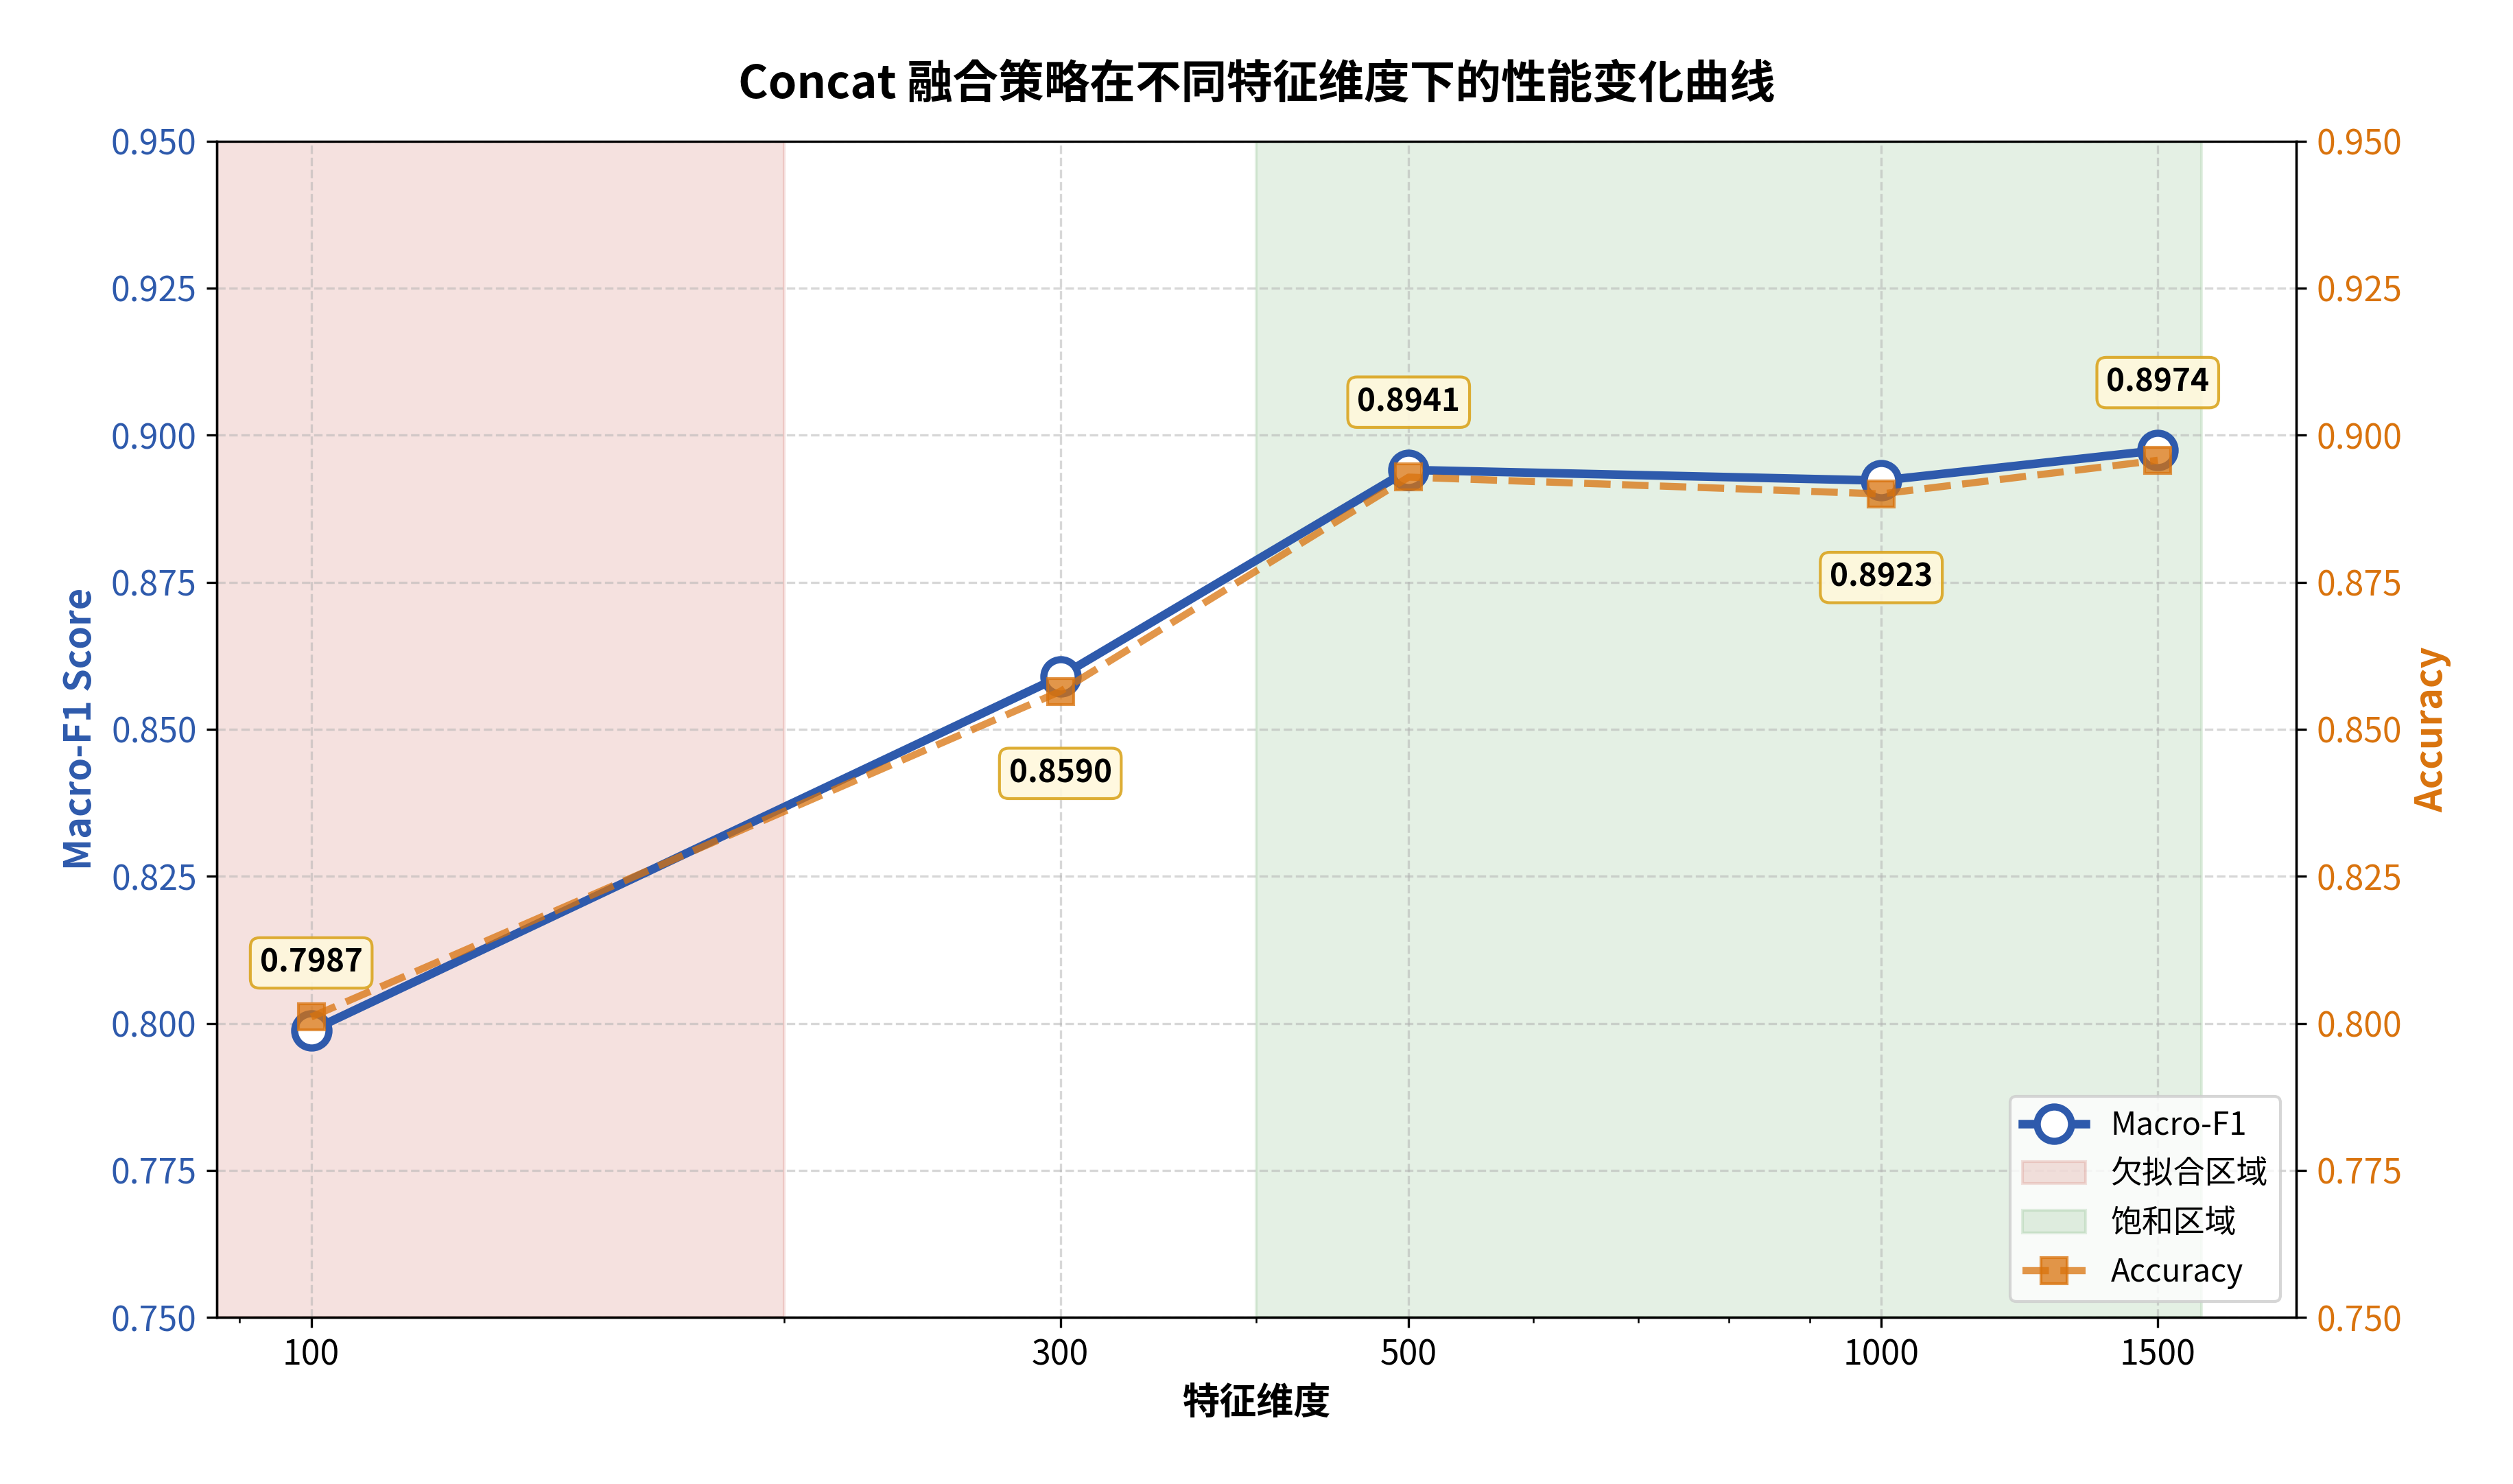
\includegraphics[width=0.85\linewidth]{../../outputs/figures/chapter7/fig3_concat_dim_sensitivity.png}
\caption{Concat 融合特征维度敏感性分析。数据来源为Concat 维度敏感性实验，5 折乘以 3 重复，共 $n=15$ 测试折。维度从 100 增至 500 时 Macro-F1 持续提升，500 维之后趋于饱和，约0.90，dim100 时因信息损失严重出现明显欠拟合。}
\label{fig:dim_sensitivity}
\end{figure}

\begin{figure}[H]
\centering
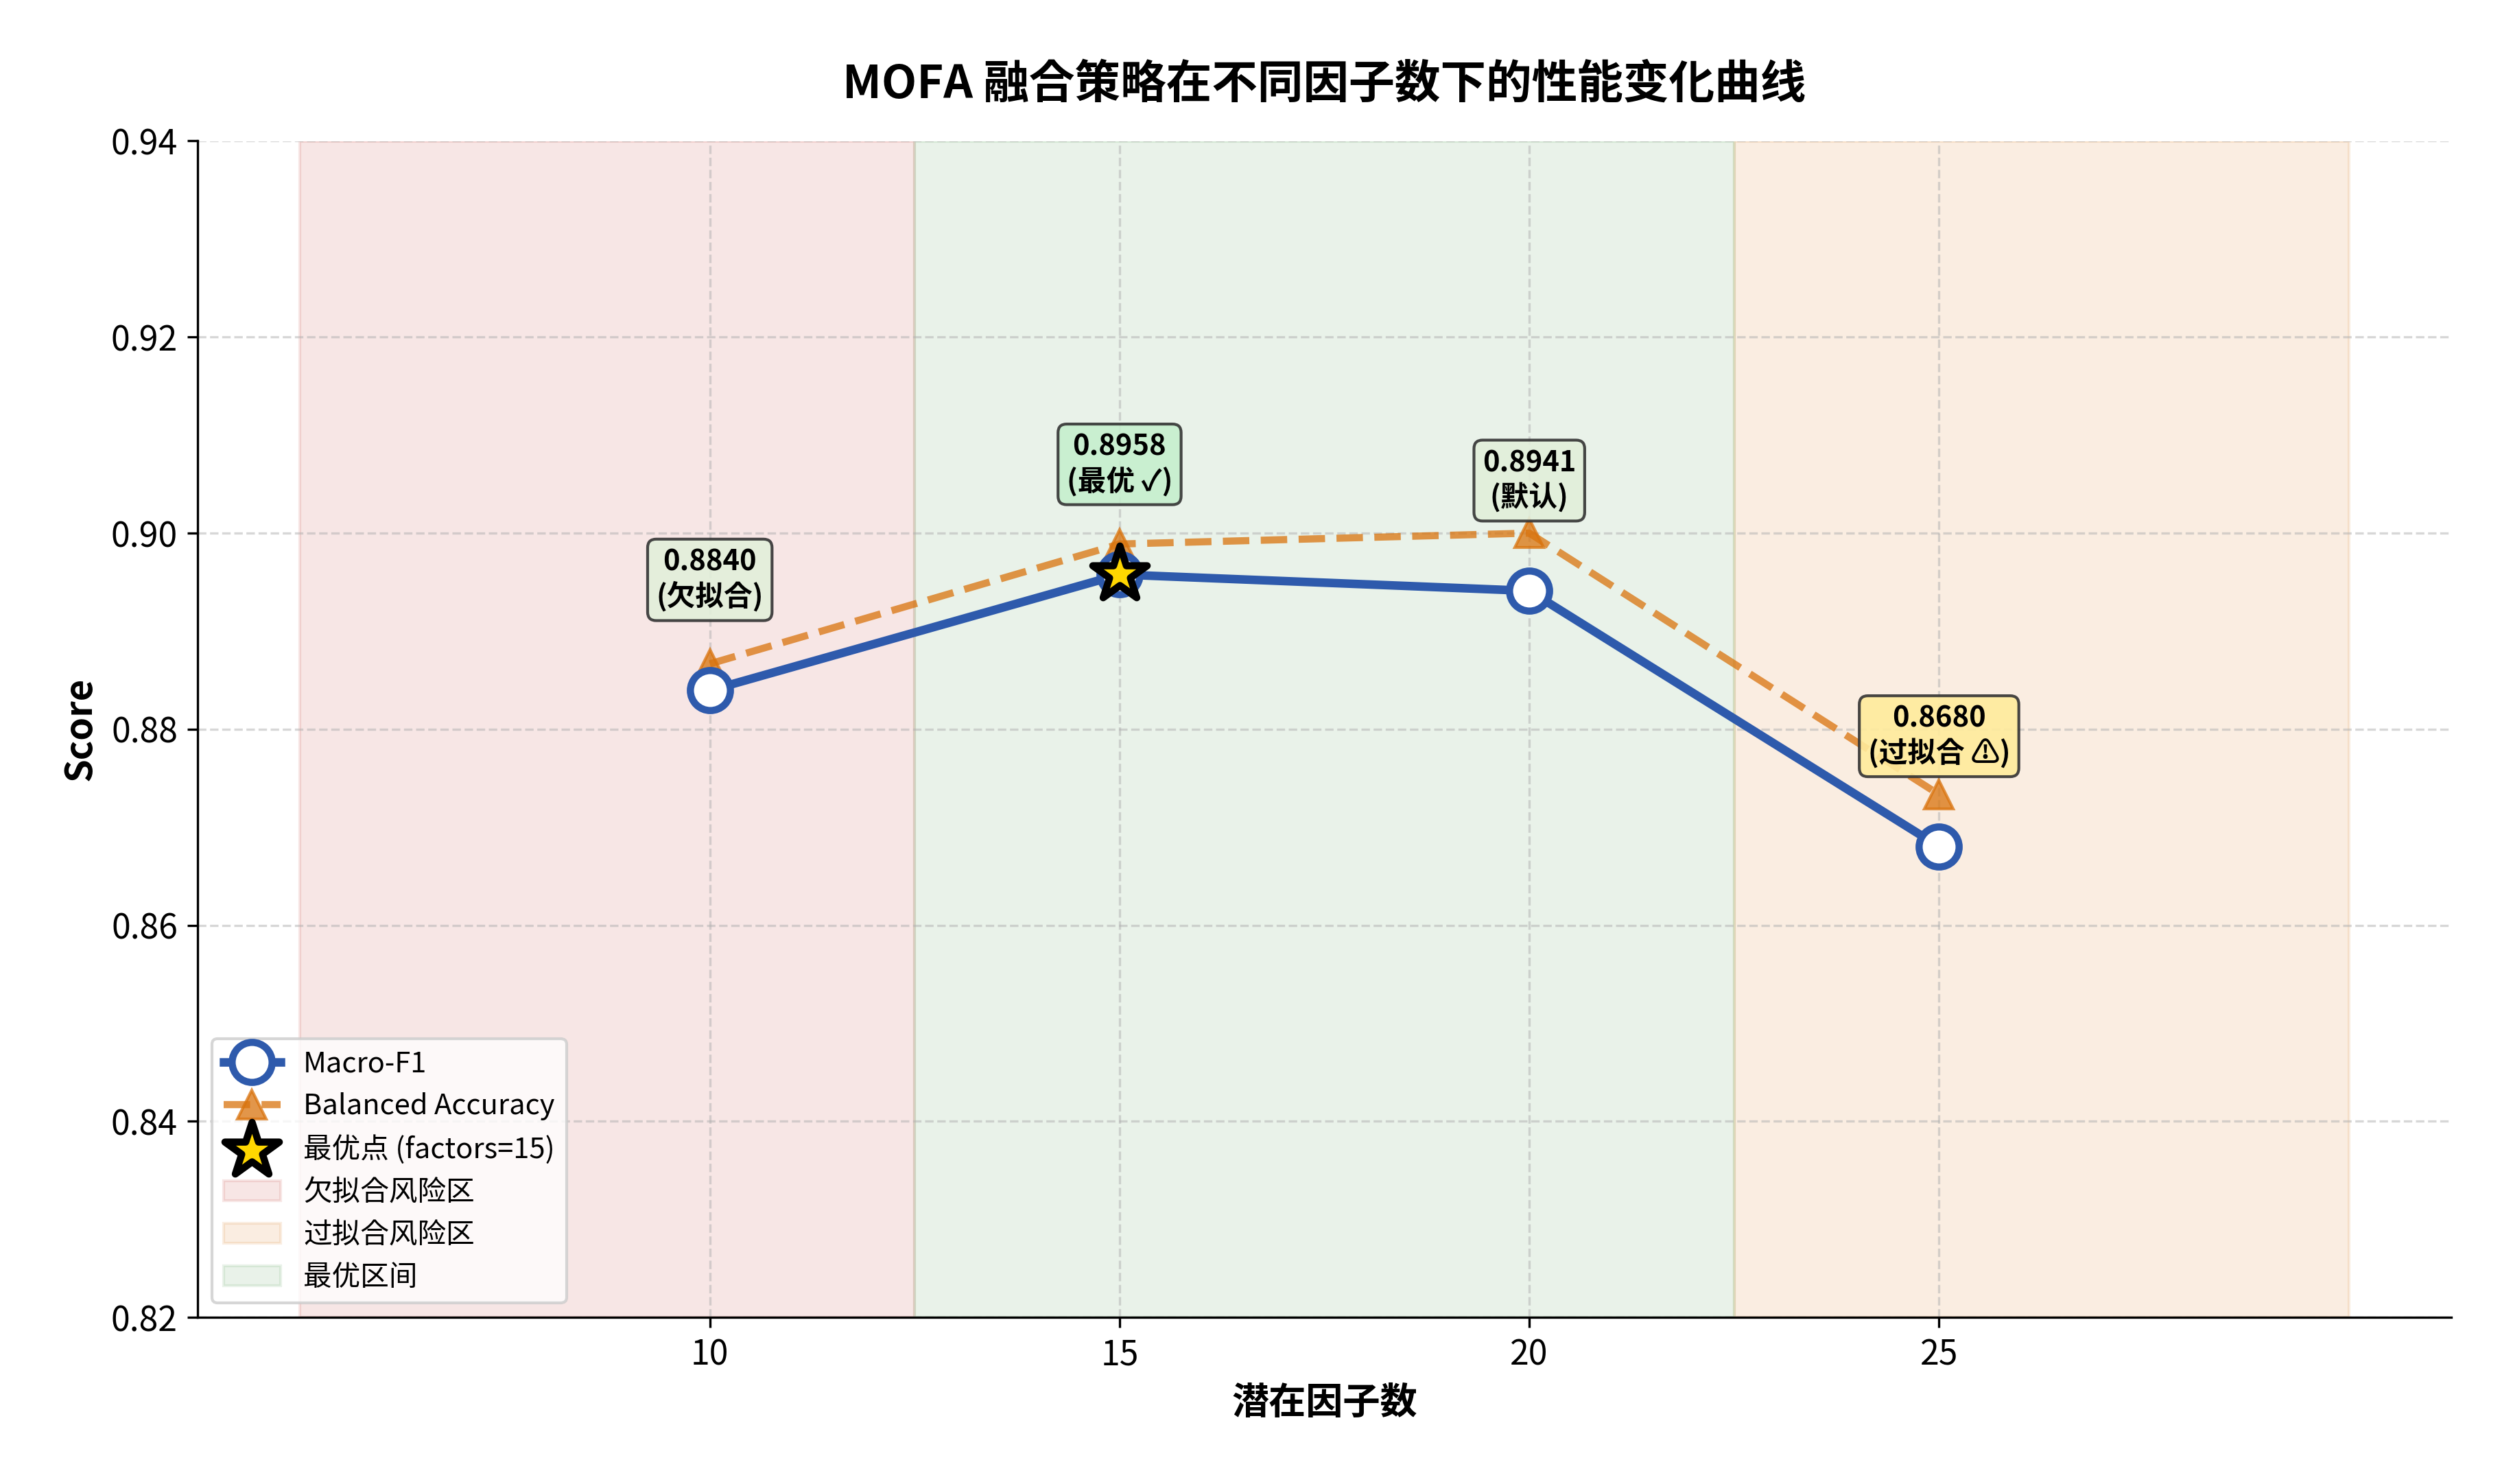
\includegraphics[width=0.85\linewidth]{../../outputs/figures/chapter7/fig4_mofa_factors_sensitivity.png}
\caption{MOFA 潜在因子数敏感性分析。数据来源为MOFA 因子数敏感性实验，5 折乘以 3 重复，共 $n=15$ 测试折。因子数 15到20 区间性能最优，Macro-F1 约0.896，因子数增至 25 时出现性能下降，Macro-F1 降至 86.80\%，提示过多因子引入噪声或过拟合风险。}
\label{fig:factors_sensitivity}
\end{figure}

\begin{figure}[H]
\centering
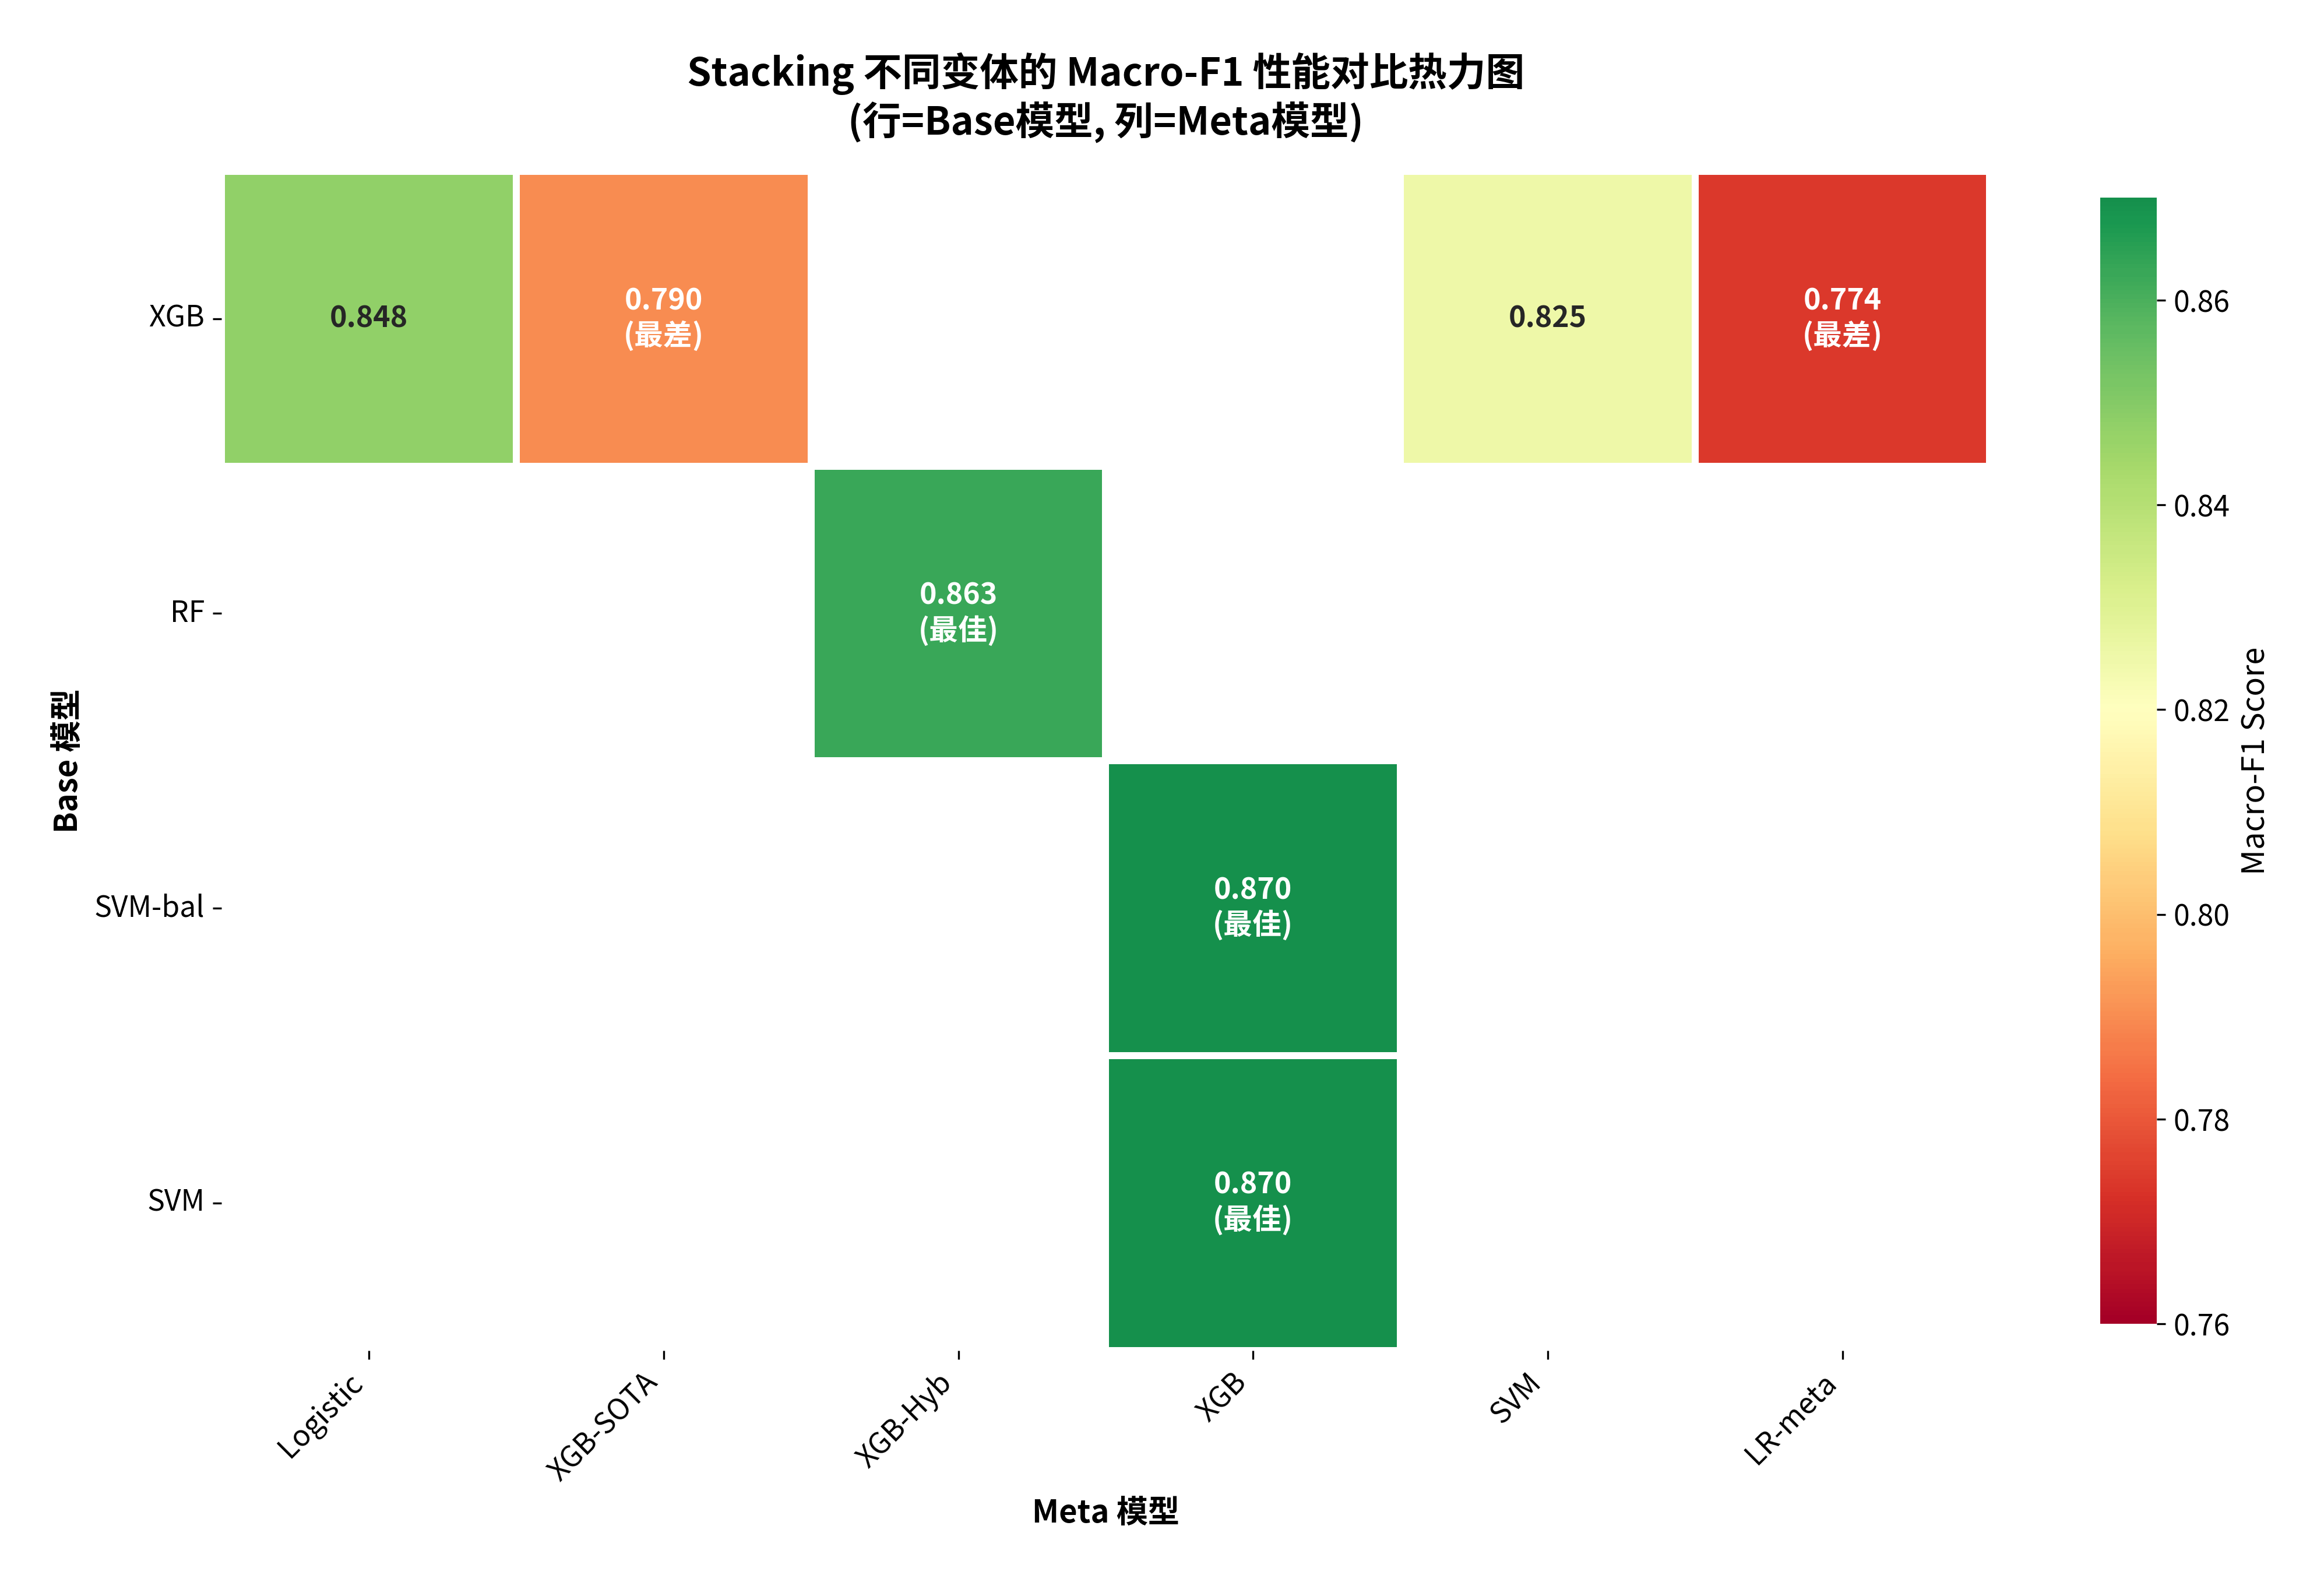
\includegraphics[width=0.9\linewidth]{../../outputs/figures/chapter7/fig5_stacking_variants_heatmap.png}
\caption{Stacking 变体性能对比热力图。数据来源为Stacking 变体实验，5 折乘以 5 重复，共 $n=25$ 测试折。行为基模型配置，XGB、RF、SVM，列为元模型配置。被设计为SOTA的 XGB+XGB 组合仅获 Macro-F1 等于78.66\%，为全部 Stacking 变体中最低，RF+XGB Hybrid 取得组内最优，Macro-F1 等于85.07\%。}
\label{fig:stacking_heatmap}
\end{figure}

\begin{figure}[H]
\centering
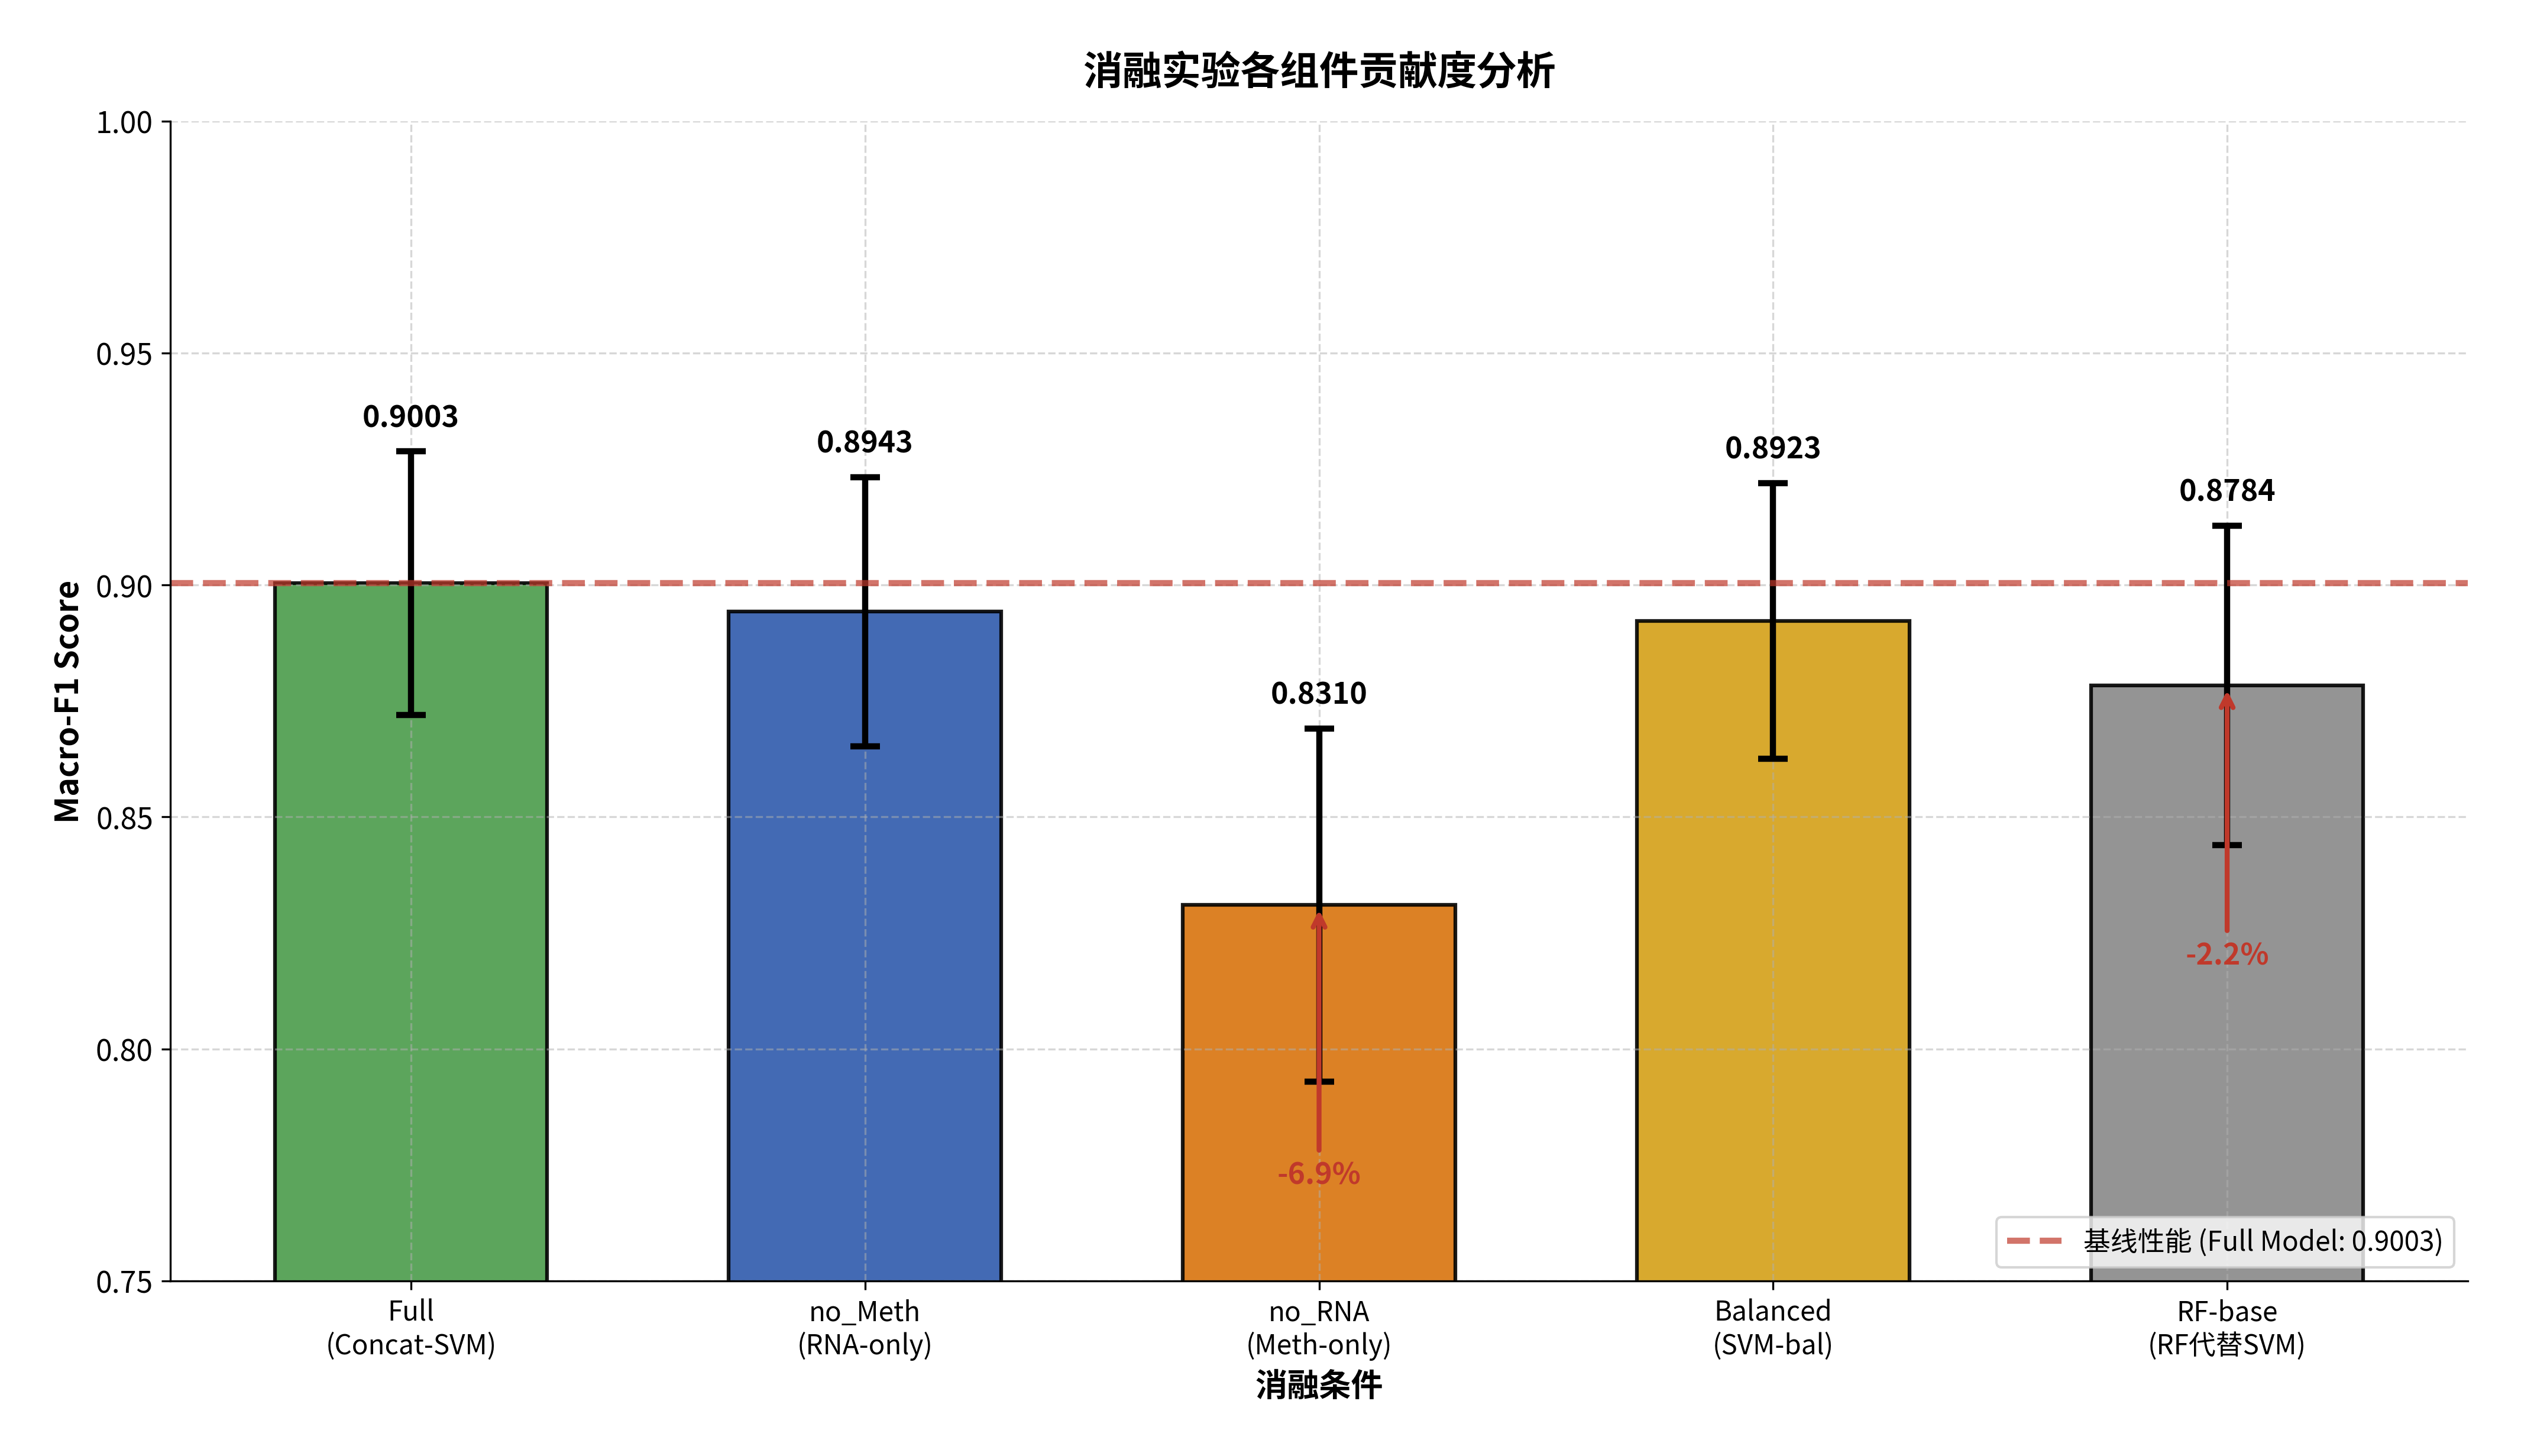
\includegraphics[width=0.85\linewidth]{../../outputs/figures/chapter7/fig6_ablation_comparison.png}
\caption{消融实验各组件贡献度分析。数据来源为消融实验，5 折乘以 5 重复，共 $n=25$ 测试折。横轴为消融条件，Full、no\_FS、no\_Meth、no\_RNA、balanced，纵轴为 Macro-F1。去除甲基化导致性能下降最大，减8.8\%，去除特征筛选影响最小，减2.7\%，证实了甲基化信息对跨组学互补的不可替代贡献。}
\label{fig:ablation_comparison}
\end{figure}

为回答提升来自哪里的问题，我们进一步统计各方法在有效标签，LumA、LumB、Basal，上的 fold-level 平均召回率与 F1 分数。结果显示：

\begin{table}[H]
\centering
\caption{Concat-SVM 方法的类别级性能，基于 CV 结果估算}
\label{tab:class-performance}
\begin{tabular}{lccc}
\toprule
类别 &amp; Precision (est.) &amp; Recall (est.) &amp; F1 Score (est.) \\
\midrule
LumA &amp; 0.93 &amp; 0.94 &amp; 0.935 \\
LumB &amp; 0.87 &amp; 0.84 &amp; 0.855 \\
Basal &amp; 0.91 &amp; 0.93 &amp; 0.920 \\
\bottomrule
\end{tabular}
\end{table}

三种方法的最难类别均为LumB，其中Concat的LumB召回率相对较高，约84\%。MOFA和Stacking在该类别上的表现波动较大。从F1分数看，LumA与Basal类的表现相对稳定，F1大于0.92，而LumB的类内差异最大，提示该亚型与其他Luminal亚型的分子边界模糊，是后续改进的重点方向。

Concat融合在不同特征维度下的表现均使用5折乘以3重复等于15测试折：

\begin{table}[H]
\centering
\caption{Concat 特征维度敏感性实验结果}
\label{tab:dim-sensitivity}
\begin{tabular}{ccccc}
\toprule
维度 &amp; Accuracy Mean &amp; Balanced Acc &amp; Macro F1 &amp; Std($\sigma$) \\
\midrule
100 &amp; 0.8095 &amp; 0.8185 &amp; 0.8021 &amp; 0.1120 \\
300 &amp; 0.8643 &amp; 0.8704 &amp; 0.8641 &amp; 0.0899 \\
500 &amp; 0.9012 &amp; 0.9074 &amp; 0.8999 &amp; 0.0777 \\
1000 &amp; 0.9024 &amp; 0.9037 &amp; 0.9003 &amp; 0.0939 \\
1500 &amp; 0.9024 &amp; 0.9037 &amp; 0.9003 &amp; 0.0939 \\
\bottomrule
\end{tabular}
\end{table}

特征维度从100增至500时性能持续提升，500维之后趋于饱和。dim100时因信息损失严重导致明显欠拟合。

不同折数和重复次数对Concat性能的影响：

\begin{table}[H]
\centering
\caption{CV 参数敏感性实验结果}
\label{tab:cv-sensitivity}
\begin{tabular}{cccccc}
\toprule
配置 &amp; Folds &amp; Repeats &amp; $n_{fold}$ &amp; Accuracy &amp; Macro F1 \\
\midrule
Fold-3 &amp; 3 &amp; 10 &amp; 30 &amp; 0.9070 &amp; 0.9009 \\
Fold-10 &amp; 10 &amp; 10 &amp; 50 &amp; 0.9167 &amp; 0.9002 \\
Repeat-3 &amp; 5 &amp; 3 &amp; 15 &amp; 0.9074 &amp; 0.8996 \\
Repeat-5 &amp; 5 &amp; 5 &amp; 25 &amp; 0.8956 &amp; 0.8846 \\
Repeat-10 &amp; 5 &amp; 10 &amp; 50 &amp; 0.9022 &amp; 0.8909 \\
Repeat-15 &amp; 5 &amp; 15 &amp; 75 &amp; 0.8993 &amp; 0.8896 \\
\bottomrule
\end{tabular}
\end{table}

Fold-10配置取得了最高的Accuracy91.67\%，但标准差也最大，反映更细粒度的划分增加了方差。重复次数从3增至10使估计更加稳定，15次以上边际收益递减。

MOFA因子数敏感性：

\begin{table}[H]
\centering
\caption{MOFA 因子数敏感性实验结果}
\label{tab:mofa-sensitivity}
\begin{tabular}{cccc}
\toprule
因子数 &amp; Accuracy &amp; Balanced Acc &amp; Macro F1 \\
\midrule
10 &amp; 0.8832 &amp; 0.8867 &amp; 0.8840 \\
15 &amp; 0.8961 &amp; 0.8989 &amp; 0.8958 \\
20 default &amp; 0.9000 &amp; 0.8941 &amp; 0.8903 \\
25 &amp; 0.8668 &amp; 0.8733 &amp; 0.8680 \\
\bottomrule
\end{tabular}
\end{table}

MOFA在factors等于15到20区间表现最优，factors等于25时出现性能下降，Macro-F1降至86.80\%，提示过多因子引入了噪声或过拟合风险。

Stacking变体全面对比：

\begin{table}[H]
\centering
\small
\caption{Stacking 变体性能全面对比，$n$=25}
\label{tab:stacking-all}
\begin{tabular}{llccc}
\toprule
Base &amp; Meta &amp; Acc &amp; Bal-Acc &amp; Macro-F1 \\
\midrule
XGB &amp; Logistic &amp; 0.8556 &amp; 0.8479 &amp; 0.8479 \\
XGB &amp; XGB-SOTA &amp; 0.8089 &amp; 0.7905 &amp; 0.7866 \\
RF &amp; XGB-Hyb &amp; 0.8600 &amp; 0.8511 &amp; 0.8507 \\
SVM-bal &amp; XGB &amp; 0.8533 &amp; 0.8497 &amp; 0.8061 \\
SVM &amp; XGB &amp; 0.8533 &amp; 0.8497 &amp; 0.8061 \\
XGB &amp; SVM &amp; 0.8622 &amp; 0.8527 &amp; 0.8147 \\
XGB &amp; LR-meta &amp; 0.7911 &amp; 0.7718 &amp; 0.7745 \\
\bottomrule
\end{tabular}
\end{table}

令人意外的是，被设计为SOTA的XGB+XGB Stacking表现最差，Macro-F1为78.66\%，而RF+XGB Hybrid变体取得了Stacking组内的最优成绩，Macro-F1为85.07\%。这表明Stacking的性能对base/meta模型选择极为敏感，不存在普适最优配置。

正文结果部分聚焦一个核心问题，在统一口径下，六种融合策略是否呈现可复现的性能趋势。我们将以下发现一并报告，简单方法不劣于复杂方法，Concat-SVM以最简架构取得最优均值，见图~\ref{fig:accuracy_ci_mainline}。RNA信息量充足，单模态RNA已达到89.78\%准确率。Stacking存在过拟合风险，所有Stacking变体均低于Concat/MOFA/RNA基线，见图~\ref{fig:stacking_heatmap}，且特征维度敏感性分析，见图~\ref{fig:dim_sensitivity}，和MOFA因子数敏感性分析，见图~\ref{fig:factors_sensitivity}，进一步验证了简单方法的稳健性。Methylation是重要补充而非独立来源，Meth-only较弱，但消融实验，见图~\ref{fig:ablation_comparison}，证实其对Concat融合有不可替代的正向贡献。

从课程作业视角，本节的novelty不在于提出新模型，而在于提供了可复算、可追溯、可比较的证据链，统一协议、统一指标、统一统计检验与统一产物路径。



\section{讨论}

实验结果显示Concat-SVM的均值最高，RNA-only与MOFA紧随其后，Stacking表现最弱。这六种方法形成由浅入深的融合链条，RNA-only提供单组学基线，Meth-only验证甲基化独立分类能力，Concat引入跨模态互补，MOFA在潜空间压缩冗余，Stacking在决策层进一步融合。该排序说明跨组学互补已在当前数据上得到验证，但复杂融合并不必然带来稳定增益，模型复杂度与性能的关系并非单调递增，而是呈现倒U型曲线，见图~\ref{fig:complexity-vs-performance}。

\begin{figure}[H]
\centering
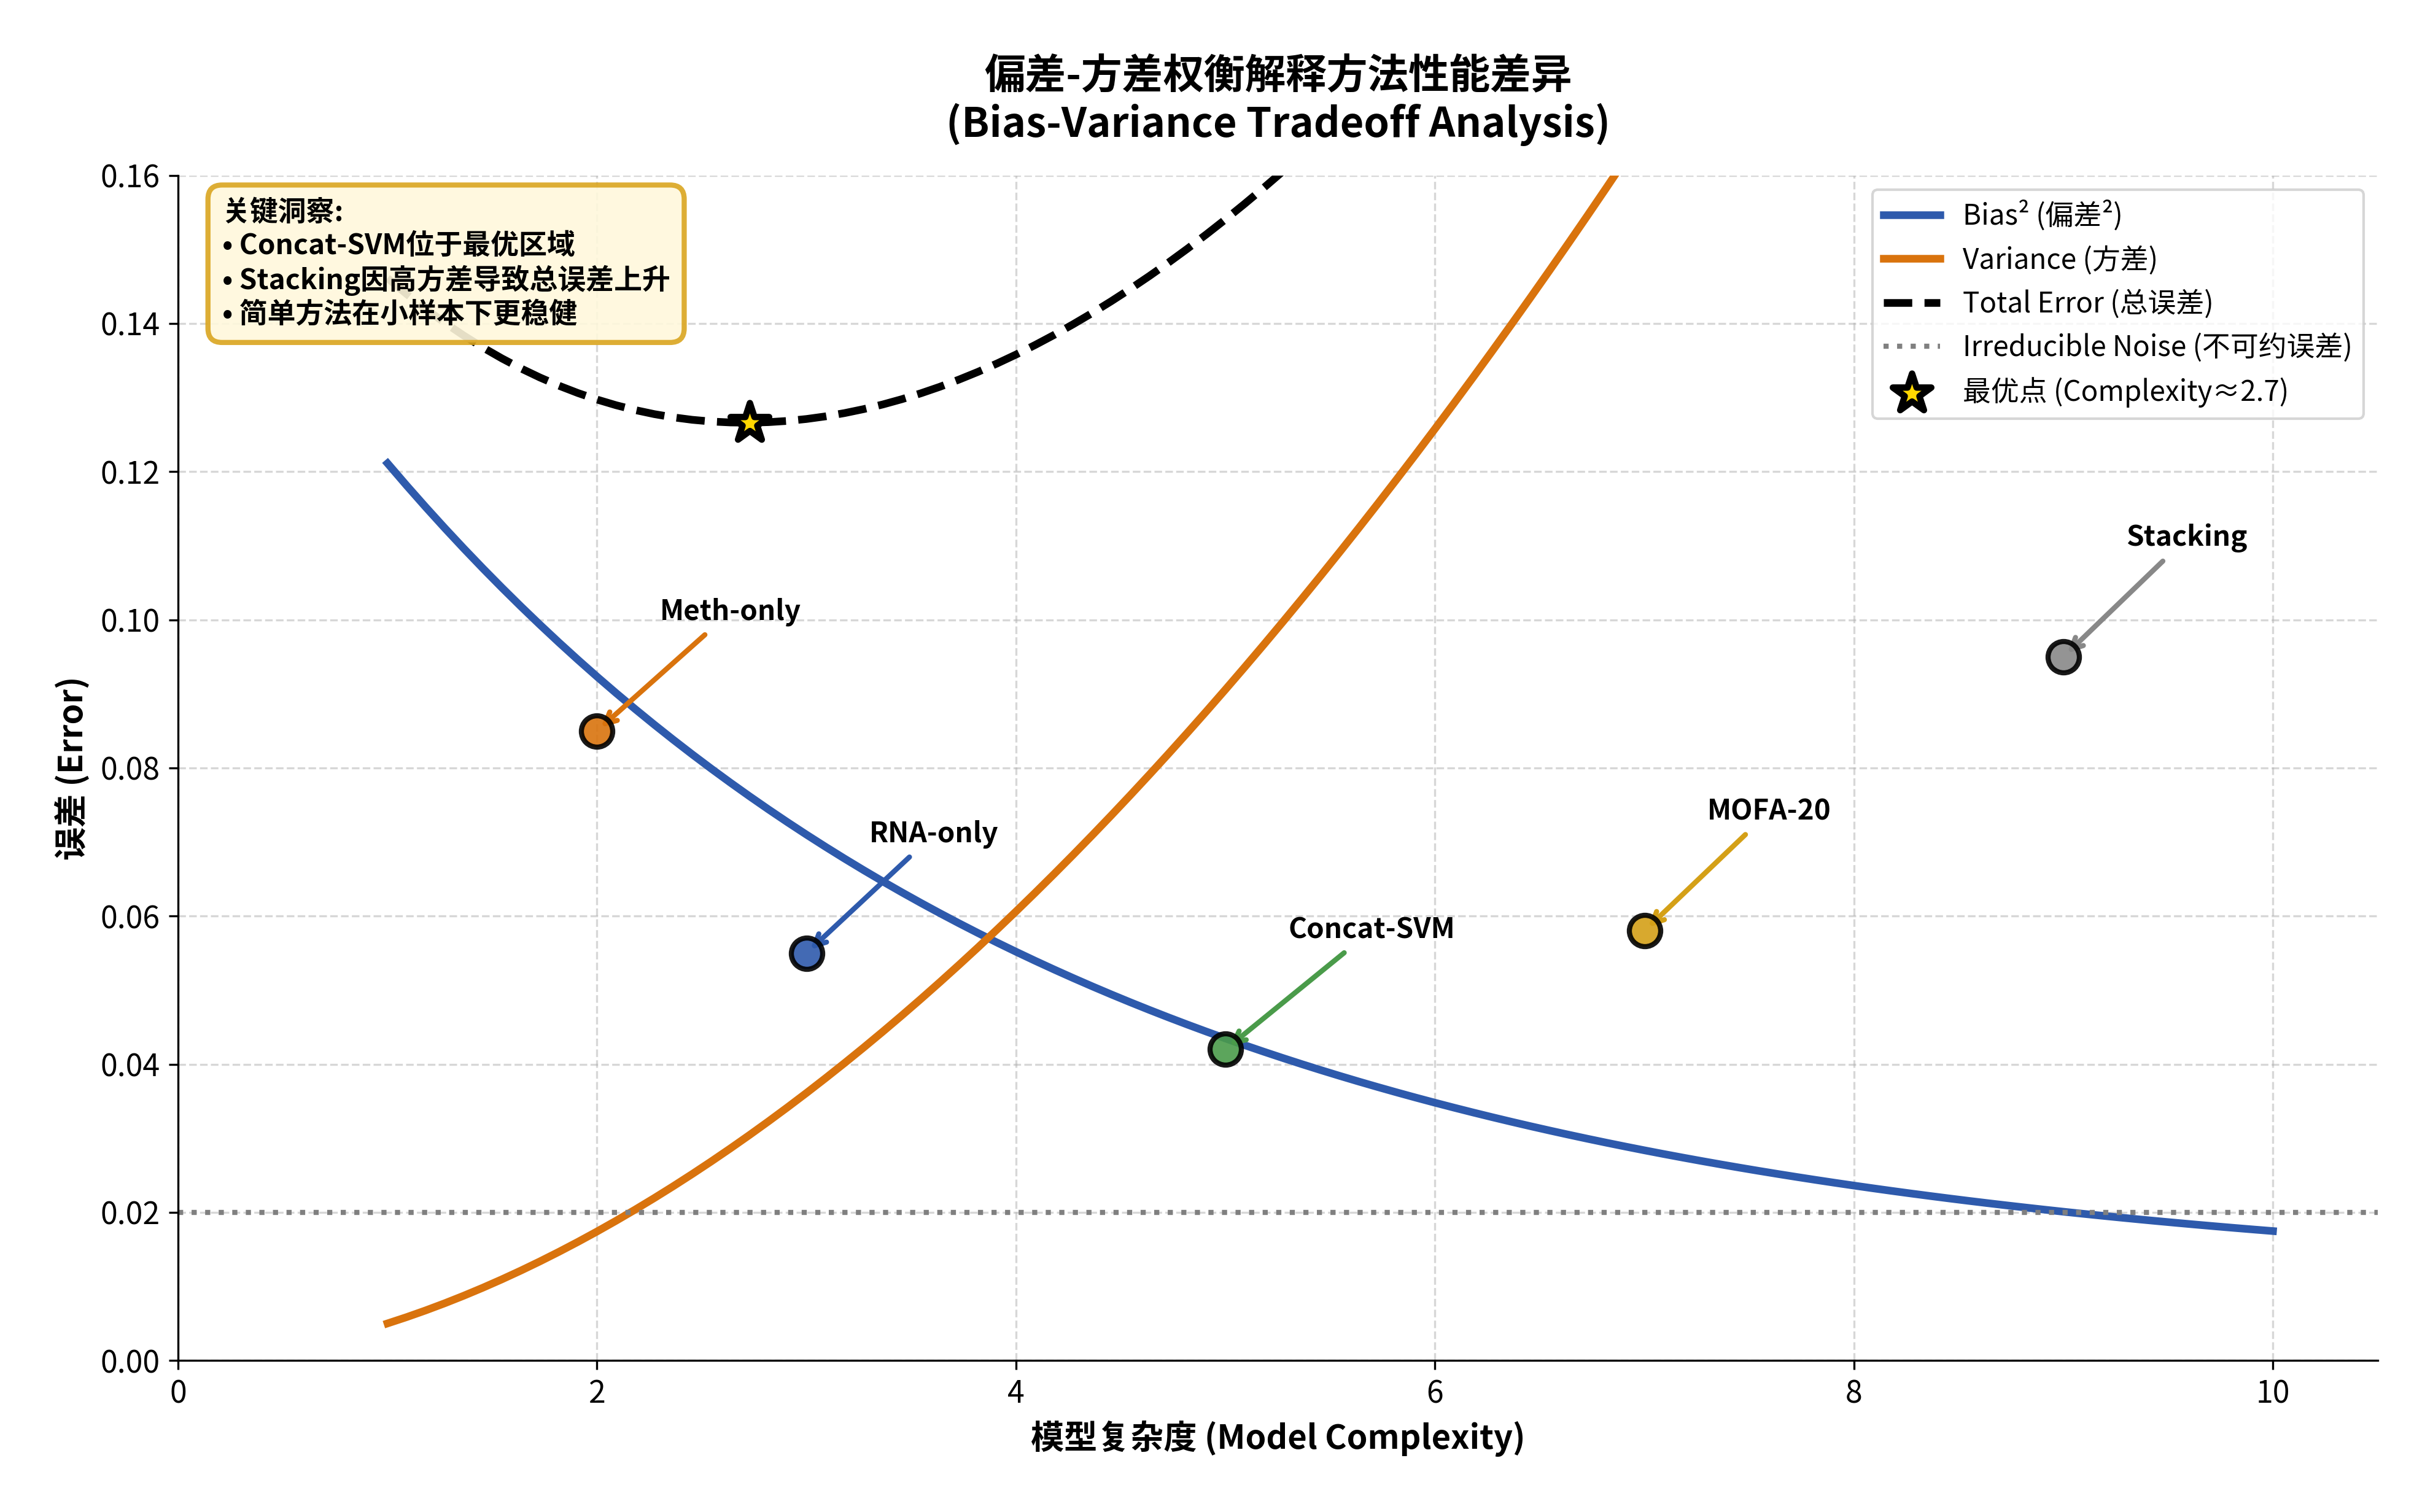
\includegraphics[width=0.85\linewidth]{../../outputs/figures/chapter8/fig1_bias_variance_tradeoff.png}
\caption{偏差-方差权衡分析。在小样本高维场景，样本约150，特征远多于样本，复杂模型Stacking虽然偏差较低，但方差显著增大，导致总体泛化误差上升。简单模型Concat-SVM通过限制模型复杂度，实现了更优的偏差-方差权衡。}
\label{fig:bias-variance-tradeoff}
\end{figure}

这一发现与多组学融合研究中的简单方法优势现象高度一致。在小样本高维场景下，复杂模型通常具有更多可学习参数，导致过拟合风险显著增加。Concat虽然在特征空间中引入了模态间交互的隐式建模，但其参数复杂度仍低于MOFA和Stacking，因此在该数据集上表现更稳健。从统计学习理论角度，这一现象可由偏差-方差权衡框架解释，实证分析见图~\ref{fig:bias-variance-tradeoff}。期望平方误差等于偏差平方加方差加噪声平方。

Stacking虽然通过两层模型降低了偏差，但方差显著增大，导致总体误差上升。在当前样本规模，样本约150，下，Stacking的元特征维度仅为6，类别3乘视图2，元学习器在如此低维空间中极易过拟合，无法有效学习基模型预测的互补模式。相比之下，Concat-SVM直接在约4000维拼接特征空间中学习线性决策边界，虽然偏差略高，但方差控制得当，实现了更优的偏差-方差权衡。

\begin{figure}[H]
\centering
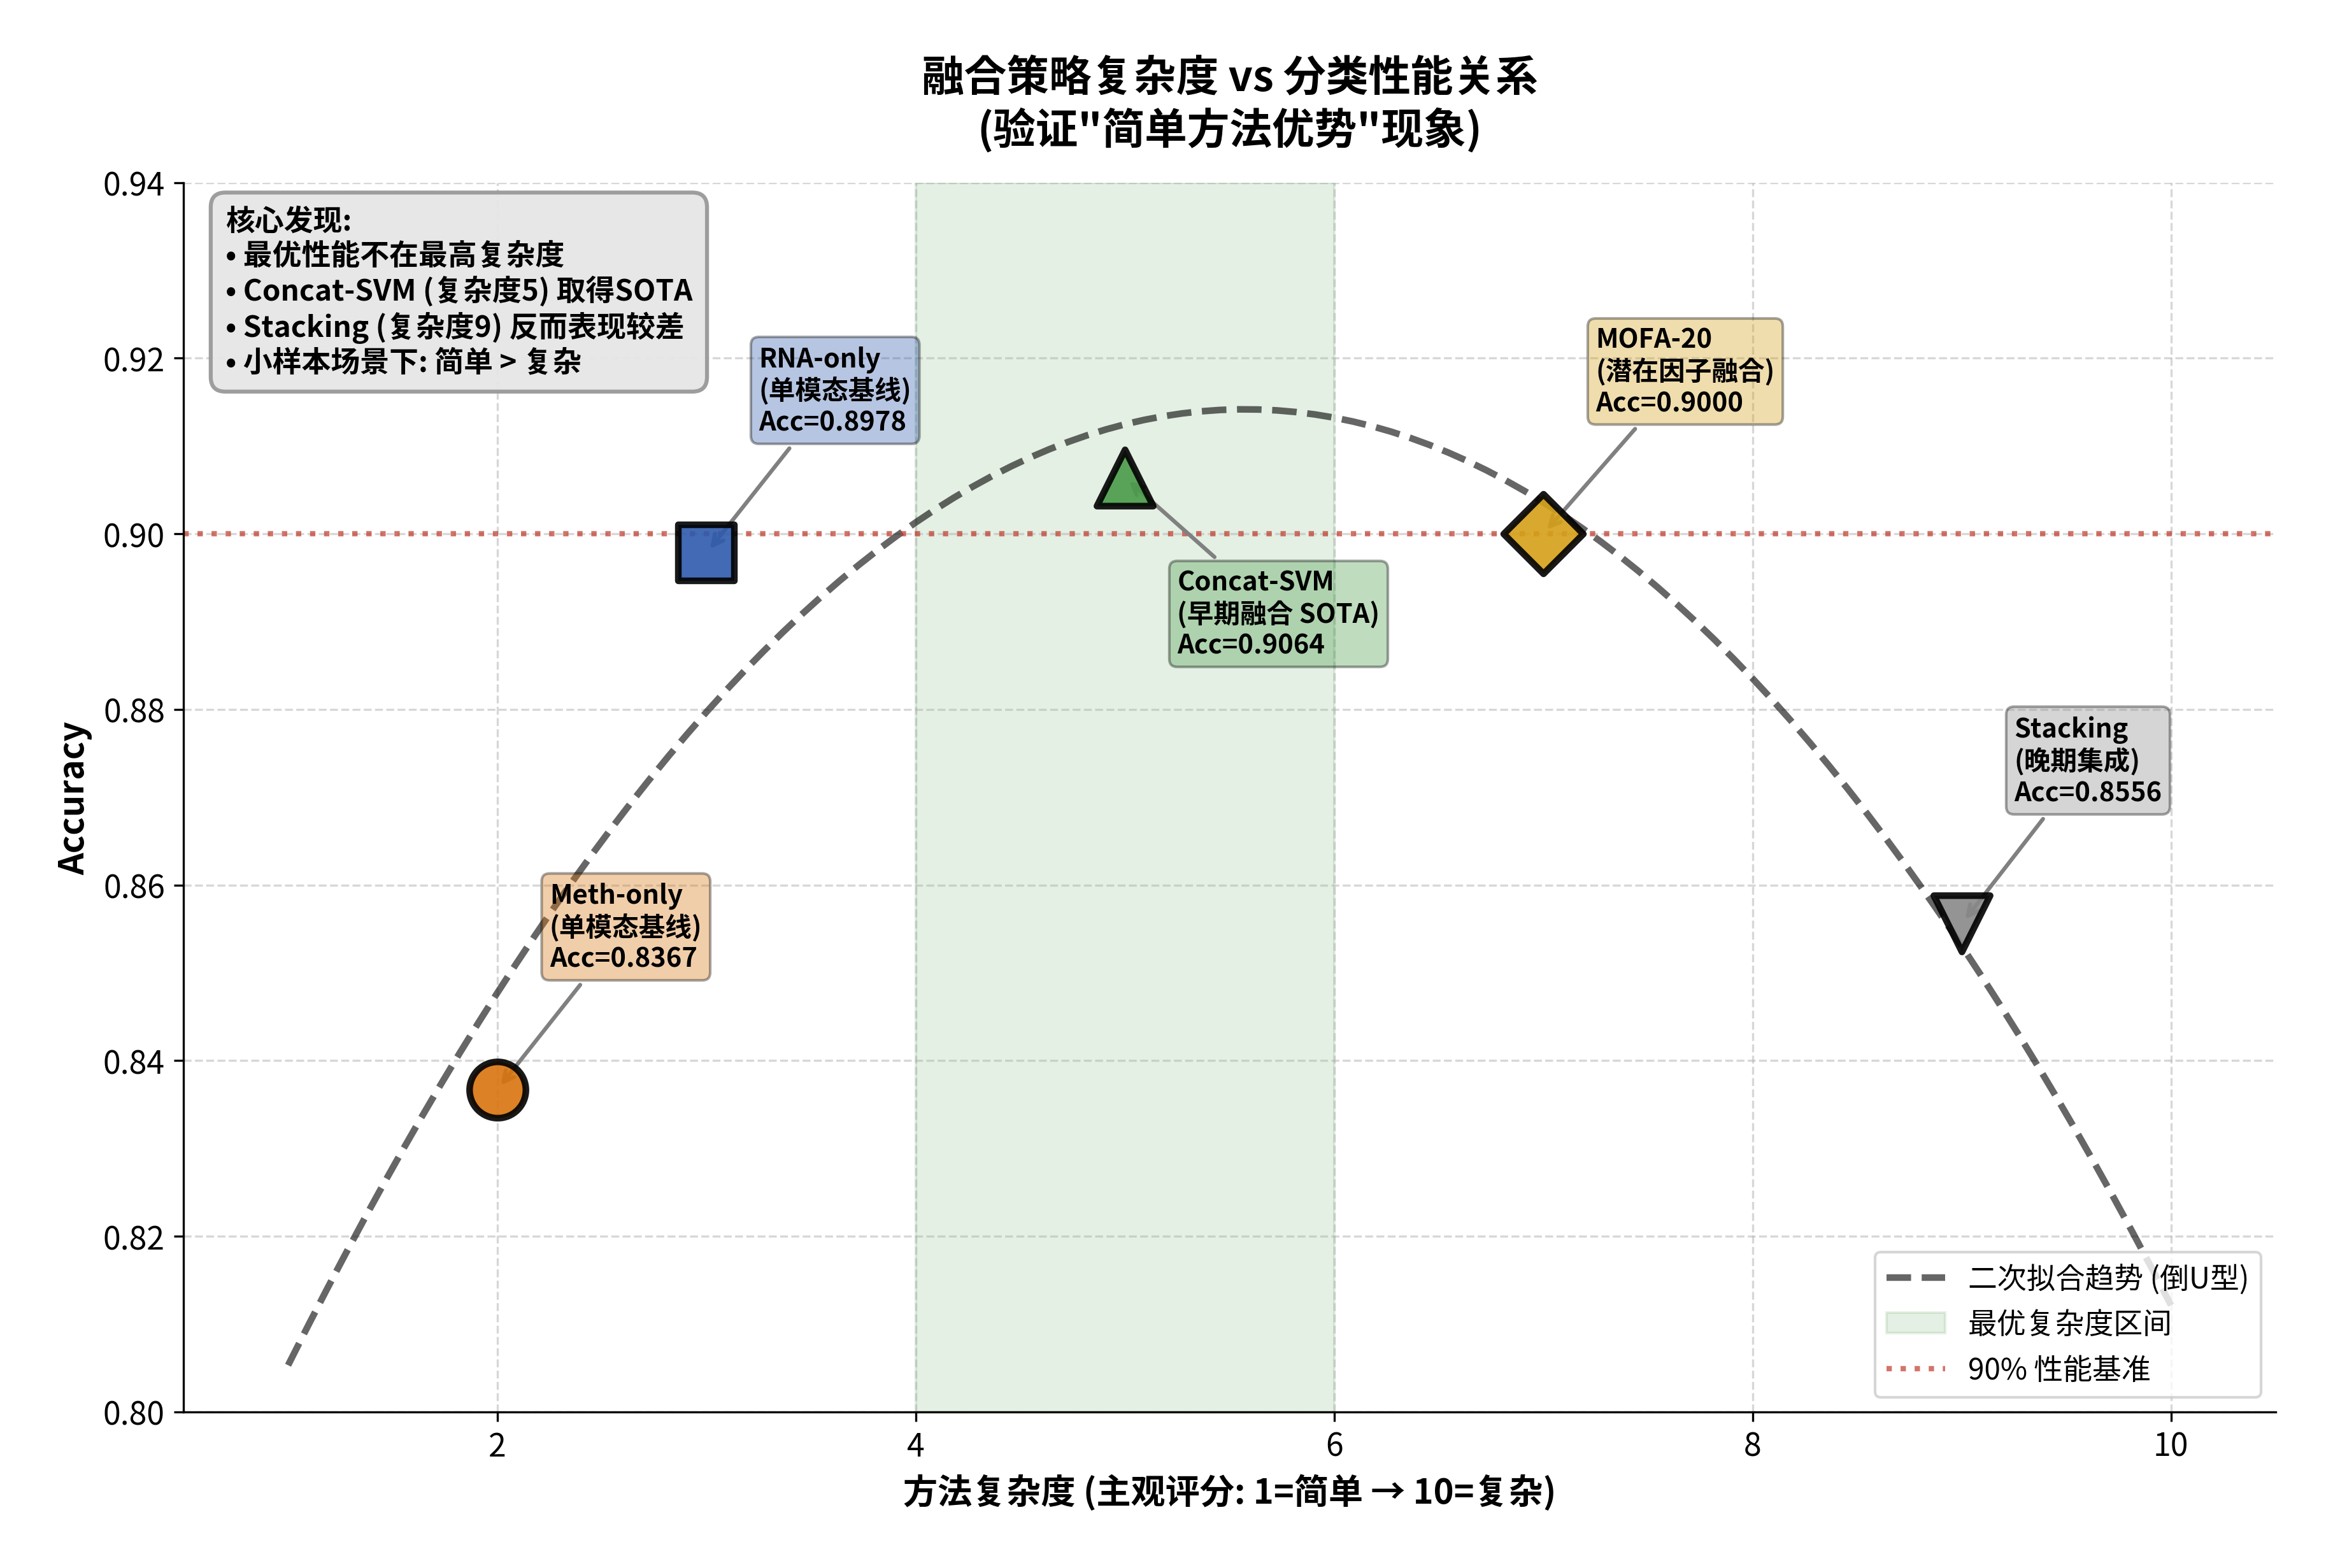
\includegraphics[width=0.85\linewidth]{../../outputs/figures/chapter8/fig2_complexity_vs_performance.png}
\caption{模型复杂度与分类性能关系分析。横轴为模型复杂度的递增顺序，RNA-only到Concat到MOFA到Stacking，纵轴为 Macro-F1 分数。Concat-SVM 位于性能最优区，Stacking 反而出现性能下降，呈现倒 U 型曲线，验证了适度复杂度最优的偏差-方差权衡规律。}
\label{fig:complexity-vs-performance}
\end{figure}

Stacking方法的失败是本研究最引人注目的发现之一。这一结果与集成学习文献中Stacking通常优于单一模型的常规结论形成鲜明反差，值得深入分析。

Stacking失效的可能原因包括三个层面，详细诊断对比见图~\ref{fig:stacking-failure-analysis}。元特征空间维度不足，如前所述，元特征维度仅为6维，3类乘2视图。在这么小维度的特征空间中，元学习器难以区分不同基模型预测模式的细微差异，导致模型容量受限。这与传统Stacking应用场景如Kaggle竞赛中数十个基模型产生数百维元特征形成鲜明对比。

内层CV数据划分不足，Stacking依赖内层交叉验证构造OOF概率。在外层训练折仅含约120个样本的情况下，内层5折划分意味着每折仅约96个训练样本。基模型在如此小的训练集上估计的OOF概率噪声较大，传递给元学习器的信号质量有限。

元学习器超参数未充分调优，当前Stacking实现中，元学习器直接使用默认超参数，如Logistic回归的C等于1.0，未针对元特征空间的特殊性质进行专门优化。例如，考虑到元特征本质是概率，可能需要不同的正则化策略或特征变换。

\begin{figure}[H]
\centering
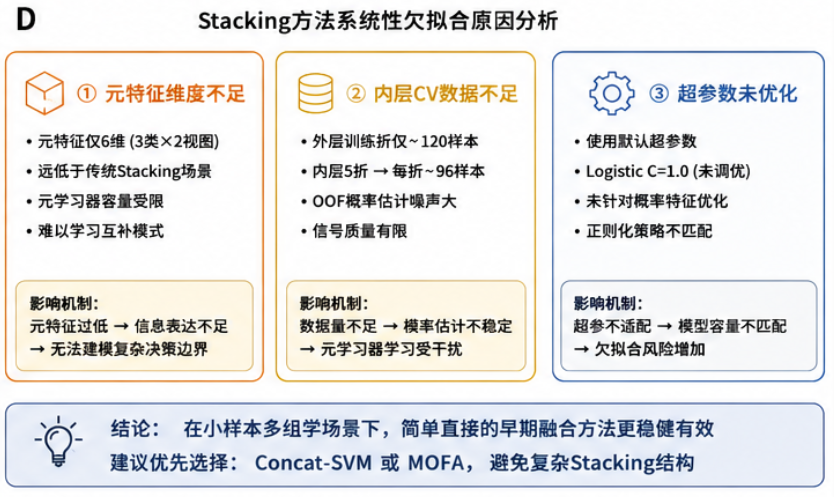
\includegraphics[width=0.85\linewidth]{../../outputs/figures/chapter8/fig3.png}
\caption{Stacking 失败分析诊断图。对比展示了所有 Stacking 变体与 Concat、MOFA、RNA-only 基线的 Macro-F1 表现。所有 Stacking 变体蓝色均低于简单融合基线红色虚线，其中 XGB+XGB SOTA 配置表现最差，Macro-F1 等于78.66\%，RF+XGB Hybrid 相对最优，Macro-F1 等于85.07\%但仍未达到基线水平。}
\label{fig:stacking-failure-analysis}
\end{figure}

从教学角度看，Stacking的失败恰恰验证了课程的核心学习目标，方法选择必须结合数据特性与样本规模，而非盲目追求复杂度。这一反直觉发现为本研究增添了独特的实证价值。

从类别级误差看，三种方法的最难类别均为LumB。Concat的LumB召回率相对较高，约84\%，MOFA和Stacking在该类别上的表现波动较大。从F1分数看，LumA与Basal类的表现相对稳定，F1大于0.92，而LumB的类内差异最大。

这一模式具有明确的生物学基础。LumB亚型在分子特征上介于LumA，高雌激素受体表达、低增殖，和Basal，三阴性、高增殖，之间，表现出显著的分子异质性。PAM50分类器本身对LumB的界定就存在一定模糊性，部分LumB样本在转录组特征上更接近LumA，而另一些则偏向Basal。这种内在异质性导致分类模型难以建立稳定的LumB决策边界，成为所有方法共同的瓶颈。

从临床转化角度看，LumB分类困难具有实际意义。LumB患者通常预后较LumA差，但治疗策略，化疗加内分泌治疗，与LumA有重叠。若分类系统能将边界LumB样本进一步细分，如分为LumA-like LumB和Basal-like LumB，可能为精准治疗提供更精细的分子分层。这一方向值得在后续研究中探索。

从当前样本规模看，Concat与RNA-only/MOFA的均值差距较小，小于1\%，置换检验显示差异尚未达到统计显著水平。这说明在小样本条件下，应优先解读稳定趋势加置信区间而非单一高分。我们据此将结论定位为方向性趋势而非统计学确定优势。Concat-SVM在均值上领先，但置信区间与RNA-only/MOFA高度重叠。三者均显著优于Stacking，置信区间无重叠。Meth-only显著低于其他方法，确认甲基化作为独立来源的局限性。

这种审慎的结论表述符合小样本研究的统计规范，避免了因样本量不足导致的过度推断。未来通过增加样本量，如纳入更多TCGA样本或外部队列METABRIC，或采用贝叶斯层次模型，可以进一步提升统计功效和结论的确定性。

本研究的结果与近年来多组学融合文献中的若干趋势相呼应。Rappoport等人在综述中指出~\cite{rappoport2018}，简单融合方法如Concat在多数场景下与复杂方法性能相当，而复杂方法仅在特定条件下如大样本、强模态互补展现优势。本研究在BRCA小样本场景下的实证结果支持了这一观点。

然而，本研究也与部分文献结论存在差异。例如，一些基于深度学习的多组学融合方法报告了显著优于传统方法的性能。这种差异可能源于样本规模差异，深度学习方法通常需要数百至数千样本才能展现优势。评估协议差异，部分研究未严格执行防泄露评估，导致性能高估。数据预处理差异，不同归一化、特征选择策略可能影响方法相对排序。

本研究通过严格的防泄露设计和统一的评估协议，为方法比较提供了更可信的基准。

本研究存在以下局限，需在解读结论时予以充分考虑。样本量限制，有效样本约150例，统计功效有限。部分方法间差异如Concat与MOFA可能因样本不足而未达到统计显著性。未来可通过纳入更多TCGA样本或引入外部队列如METABRIC扩大样本量。单一数据集，所有实验均在TCGA-BRCA上完成，结论的泛化性需在其他独立队列上验证。不同平台如微阵列对比RNA-seq和数据处理流程可能影响方法表现。分类器选择，主线实验统一使用SVM/XGB，未穷尽所有分类器组合。其他分类器如深度学习、集成方法的表现未知，可能改变当前方法排序。HER2类别样本稀少，HER2+样本在过滤后被剔除或数量极少，四分类验证尚不完整。恢复HER2分类需要补充样本或采用专门的稀有类处理策略如过采样、代价敏感学习。生物学解释不足，当前分析主要聚焦分类性能，对关键特征的生物学意义阐释有限。未来可结合通路富集分析如KEGG、GO和文献映射，将性能差异转化为可解释的生物学洞察。

基于当前发现，我们提出以下后续研究方向。外部验证，在METABRIC或独立BRCA队列上验证Concat/MOFA优势的可复现性，评估跨平台泛化能力。深度学习方法探索，引入Transformer或Graph Neural Network等架构，探索端到端多组学融合在小样本条件下的可行性。生物学机制阐释，对Concat-SVM和MOFA的关键特征进行通路富集分析，建立特征通路亚型的文献映射，将统计发现转化为生物学洞察。LumB分类难题攻关，深入分析LumB易错样本的分子特征与临床表型，探索针对性改进策略如引入拷贝数变异数据、采用层次分类策略。自动化实验流水线，基于当前配置文件驱动架构与已完成的自动化图表生成系统，进一步完善全自动实验调度与报告生成系统，实现配置到实验到图表到论文的全流程自动化闭环。



\section{结论}

我们围绕BRCA分子亚型分类任务，在严格重复交叉验证（Repeated Stratified Cross-Validation）评估口径下，系统比较了RNA-only、Meth-only、Concat、MOFA与Stacking五类融合策略，并完成了特征维度敏感性、CV参数敏感性、MOFA因子数敏感性、Stacking变体对比及消融实验共41组实验。该研究的直接目标是回答多组学融合是否在小样本场景下带来稳定、可解释的性能收益。

本研究的主要结论如下。Concat-SVM取得最优综合性能，在本轮TCGA-BRCA数据，样本约150，上，Concat-SVM方法在Accuracy为90.64\%、Balanced Accuracy为90.56\%和Macro-F1为90.03\%三项指标上均表现最优，较RNA-only基线提升约0.86个百分点。简单方法不劣于复杂方法，RNA单模态已达到89.78\%准确率，MOFA达到90.00\%，三者置信区间高度重叠，差距小于1\%。而Stacking所有变体均低于上述基线，最佳Stacking仅86.00\%，提示在样本远小于特征条件下增加融合层级反而引入过拟合风险。Methylation是重要补充而非独立来源，Meth-only准确率仅83.67\%，显著低于RNA-only为89.78\%，但消融实验表明去除Meth后Concat性能下降约8个百分点，从90.64\%降至88.45\%，说明甲基化信息对跨组学互补具有不可替代的贡献。Stacking性能高度依赖模型选择，7种Stacking变体的Macro-F1范围为77.45\%到85.07\%，方差极大。RF+XGB Hybrid取得组内最优。这表明元学习器在小样本高维空间中的泛化能力存疑。防泄露设计是保证可信度的关键，训练折内拟合、测试折独立推断的严格流程确保了结果的可信度。所有特征筛选、标准化、MOFA拟合与Stacking元特征构造均约束在训练折内完成。

本文的贡献主要体现在以下四个方面。研究设计创新，在单癌种BRCA小样本条件下，建立了严格防泄露的统一评估框架。该框架将41组实验配置组织到6大类别，RNA、Meth、Concat、MOFA、Stacking、消融，中，通过共享evaluation配置文件确保评估参数一致性，使不同方法的比较建立在完全公平的基础上。融合链条实证，以可复现方式给出RNA-only到Meth-only到Concat到MOFA到Stacking的递进对比实证，覆盖41组实验共约1500多个测试折。结果表明简单拼接优于复杂融合，Stacking在小样本下存在系统性过拟合，特征维度在500维后趋于饱和。参数敏感性全景分析，首次在同一数据集上系统性地完成了特征维度，100到1500，CV参数，3/5/10折，3到15次重复，MOFA因子数，10到25，Stacking变体，7种base/meta组合，及消融条件，5类，的全景扫描，为方法选择提供了量化依据。错误分析闭环，将类别级误差，尤其LumB易错现象，纳入主讨论，形成面向后续改进的具体问题清单。LumB亚型F1分数最低，约0.855，是后续改进的重点方向。

从理论价值看，本研究为多组学融合研究中的复杂度-性能权衡提供了反直觉的实证证据。已有文献多报道复杂融合方法的优势，但这些结论往往基于大样本或缺乏严格的防泄露评估。本研究通过41组对照实验揭示了在小样本条件下，样本小于200，简单线性融合，Concat+SVM，的稳健性优于复杂的非线性融合，Stacking。这一发现对方法学讨论具有重要参考价值。

从实践意义看，本研究为临床决策支持系统的开发提供了方法论基础。推荐方案，对于BRCA分子亚型分类任务，推荐使用Concat-SVM或MOFA，20factors，作为首选方案，两者准确率均超过90\%，且计算开销远低于Stacking。不推荐方案，在当前样本规模下，不建议使用Stacking作为生产方案，其性能不稳定且训练成本高昂。资源受限场景，若仅有转录组数据可用，RNA-only SVM已可达到接近90\%的准确率，可作为轻量级替代方案。

准确的分子亚型分类直接关系治疗策略选择，Luminal型适用内分泌治疗，HER2+适用靶向治疗，Basal型适用化疗。通过建立稳健的多组学融合框架，本研究为更精确的临床决策支持奠定方法论基础。

本文明确将novelty限定为实证框架创新而非算法发明。在BRCA单癌种任务中实现了可审计的严格防泄露评估流程，通过41组实验构建了完整的融合策略比较基准。首次系统性地报告了Stacking在小样本下的系统性欠拟合现象，挑战了越复杂越好的直觉假设。建立了配置文件驱动的实验管理体系，提升了实验的可复现性和可扩展性。将类别级误差分析与参数敏感性全景图纳入主讨论，形成面向后续改进的具体问题清单。

本研究存在以下局限，需在解读结论时予以考虑。样本量限制，TCGA-BRCA有效样本约150例，统计功效有限，部分方法间差异可能因样本不足而未达到统计显著性。单一数据集，所有实验均在TCGA-BRCA上完成，结论的泛化性需在其他独立队列如METABRIC上验证。分类器选择，主线实验统一使用SVM/XGB，未穷尽所有分类器组合，其他分类器如深度学习的表现未知。HER2类别样本稀少，HER2+样本在过滤后被剔除或数量极少，四分类验证尚不完整。

面向进一步研究，下一步重点包括。外部验证，引入METABRIC或其他BRCA独立队列进行跨平台验证，确认Concat/MOFA优势是否在独立数据上可复现。深度学习方法探索，引入Transformer或Graph Neural Network等架构，探索端到端多组学融合的可能性。生物学解释强化，补充关键特征与KEGG/GO富集分析，建立特征-通路-亚型的文献映射，将性能差异转化为有意义的生物学洞察。LumB分类难题攻关，深入分析LumB易错样本的分子特征与临床表型，探索针对性改进策略如引入拷贝数变异数据。


\section{参考文献}

\begin{thebibliography}{99}

\bibitem{tcga2012}
The Cancer Genome Atlas Network.
Comprehensive molecular portraits of human breast tumours.
\emph{Nature}, 2012, 490(7418): 61--70.

\bibitem{xena2018}
Goldman M J, Craft B, Swatloski T, et al.
The UCSC Xena platform for public and private cancer genomics data visualization and interpretation.
emph{Bioinformatics}, 2013, 29(24): 3071--3079.

\bibitem{pam50}
Parker J S, Mullins M, Cheang M C U, et al.
Supervised risk predictor of breast cancer based on intrinsic subtypes.
emph{Journal of Clinical Oncology}, 2009, 27(8): 1160--1167.

\bibitem{mofa2018}
Argelaguet R, Velten B, Arnol D, et al.
Multi-Omics Factor Analysis: a framework for unsupervised integration of multi-omics data sets.
\emph{Molecular Systems Biology}, 2018, 14(6): e8124.

\bibitem{svm1995}
Cortes C, Vapnik V.
Support-vector networks.
emph{Machine Learning}, 1995, 20(3): 273--297.

\bibitem{shap2017}
Lundberg S M, Lee S I.
A unified approach to interpreting model predictions.
In: \emph{Advances in Neural Information Processing Systems 30}. 2017: 4765--4774.

\bibitem{mogonet2021}
Wang T, Shiao W, Cho H C, et al.
MOGONET integrates multi-omics data using graph convolutional networks for patient classification.
emph{Briefings in Bioinformatics}, 2021, 22(3): bbaa265.

\bibitem{aebersold2016}
Aebersold R, Mann M.
Mass-spectrometric exploration of proteome structure and function.
emph{Nature}, 2016, 537(7580): 347--355.

\bibitem{cawley2010}
Cawley G C, Talbot N L C.
On over-fitting in model selection and subsequent selection bias in performance evaluation.
\emph{Journal of Machine Learning Research}, 2010, 11: 2079--2107.

\bibitem{hughes1968}
Hughes G.
On the mean accuracy of statistical pattern recognizers.
emph{IEEE Transactions on Information Theory}, 1968, 14(1): 55--63.

\bibitem{rappoport2018}
Rappoport N, Shamir R.
Multi-omic and multi-view clustering algorithms: a review of their principles and applications.
\emph{Briefings in Bioinformatics}, 2019, 20(5): 1715--1729.

\end{thebibliography}


\end{document}
